\documentclass[12pt]{article}

\usepackage[margin=1in]{geometry}
\usepackage{amsmath,amssymb,amsthm}
\usepackage{booktabs}
\usepackage{graphicx}
\usepackage{float}
\usepackage{natbib}
\usepackage{hyperref}
\usepackage{setspace}
\usepackage{array}

\setlength{\emergencystretch}{3em}
\doublespacing

\newtheorem{proposition}{Proposition}
\newtheorem{lemma}{Lemma}
\newtheorem{corollary}{Corollary}
\newtheorem{remark}{Remark}
\theoremstyle{definition}
\newtheorem{definition}{Definition}
\newtheorem{axiom}{Axiom}

\newcommand{\X}{\mathcal{X}}
\newcommand{\Y}{\mathcal{Y}}
\newcommand{\A}{\mathcal{A}}
\newcommand{\M}{\mathcal{M}}
\newcommand{\D}{\mathcal{D}}
\newcommand{\R}{\mathbb{R}}
\newcommand{\E}{\mathbb{E}}
\newcommand{\I}{I}
\newcommand{\C}{C}
\newcommand{\loss}{\ell}
\newcommand{\eps}{\varepsilon}

\title{Code Formation at Dimensional Boundaries:\\
Finite-Bandwidth Coordination and Anticipation in Biology}

\author{Ian Todd\\
Sydney Medical School\\
University of Sydney\\
Sydney, NSW, Australia\\
\texttt{itod2305@uni.sydney.edu.au}}

\date{\today}

\begin{document}

\maketitle

\begin{abstract}
A biological code is what survives when high-dimensional dynamics must coordinate through a boundary too narrow to carry them. This paper develops the claim formally. A rate-distortion and data-processing argument shows that retained low-loss protocols at finite-bandwidth boundaries take the form of finite partitions of substrate state, with fibers coherent under their assigned responses. Under finite or discretized conditions, an alternating Lloyd--Bayes improvement dynamics on encoder--decoder pairs decreases risk monotonically and has partition-shaped stationary limit points. When the substrate contains mutually action-incompatible regimes, the alphabet of any low-regret protocol is bounded below by the number of such regimes, so codes are forced rather than merely admitted; below that capacity, an explicit regret floor acts. Embedded in a small set of independently-motivated axioms about bounded self-maintenance, this conditional yields a universality theorem: any system satisfying the axioms forms a nontrivial code at one boundary. A sufficient-statistic argument extends the principle across timescales: when the substrate is entrained to a slow trajectory, anticipatory content can reside in the boundary message, in the receiver's entrained context, or in both. The operational unit is therefore the code--context pair, and stable codewords can acquire different meanings at gating events without the message itself preserving phase. A multi-layer hourglass simulator with a continuous radial dimensionality profile and a single discrete waist confirms three predictions empirically: the cardinality floor binds tightly when waist capacity falls below the action repertoire; effective dimensionality collapses smoothly from a high-dimensional bulk to a finite-alphabet waist with only partial re-expansion on the receiver side; and the task-relevant slow mode survives the waist while task-irrelevant slow modes are aliased away. The framework predicts where codes appear, where continuous coupling persists, and how channel bandwidth, slow-mode coupling, and viability pressure shape the partition. It does not derive any particular alphabet such as the codon table; it explains why such alphabets exist as a general boundary phenomenon.
\end{abstract}

\noindent\textbf{Keywords:} biological codes; code formation; dimensionality; rate-distortion; anticipation; biosemiotics

\section{Introduction}

A biological code is what survives when high-dimensional dynamics must coordinate through a boundary too narrow to carry them. Living systems are full of such codes. Nucleotide triplets map to amino acids. Spikes and oscillatory phases coordinate neural populations. Morphogens and bioelectric fields guide cell fate. Receptors and ligands mediate immune, endocrine, and developmental recognition. Bacteria use quorum-sensing molecules to coordinate population behavior. Animals compress high-dimensional bodily and social states into gestures, calls, and displays. The diversity of biological codes is not in doubt; the harder question is why coding itself appears so persistently.

Most accounts begin after codes already exist. Information theory quantifies transmission once an alphabet and channel are specified \citep{shannon1948,coverthomas2006}; biosemiotics and code biology emphasise that life depends on symbolic relations mediated by adapters and interpreters \citep{pattee1969,pattee2001,barbieri2003,barbieri2015,hoffmeyer2008,emmeche1991}; Polanyi already argued that living organisation channels chemistry by constraints not reducible to chemistry alone \citep{polanyi1968}; signalling-game theory shows how conventions stabilise once sender and receiver payoffs reward coordination \citep{lewis1969,skyrms2010}. These approaches identify essential features of codes but leave a prior constraint underdeveloped: why finite reusable alphabets should form at the boundaries of high-dimensional biological systems in the first place.

The answer proposed here is that codes form at \emph{dimensional boundaries}. A dimensional boundary is an interface at which the relevant state space on one side has more task-relevant degrees of freedom than the channel to the other side can transmit. A cell cannot transmit its full molecular state to a neighbor. A cortical area cannot transmit its full oscillatory field to a distant area through finite axons. A germline cannot transmit the full trajectory of parental physiology across generations. An organism cannot transmit its entire internal state to another organism through behavior. In each case, direct state sharing is impossible. What can cross is a compressed signal. If coordination recurs and selection favors successful compression, the signal becomes reusable: the substrate state space is partitioned into equivalence classes that preserve downstream-relevant distinctions and discard within-class variation. Such a retained stable partition is a code.

Many biological codes do more than compress: they bind fast local dynamics to slow trajectories. Circadian phase constrains metabolism before dawn; developmental stage constrains local cell decisions before the final body form exists; neural low-frequency rhythms gate high-frequency computation before behavioral commitment. In each case a system coupled to a slow variable gains anticipatory structure not by simulating future microstates but by being synchronised to a slow trajectory whose present coordinate constrains which future states are reachable. This follows Rosen's anticipatory-systems tradition and the relational accounts that develop it \citep{rosen1985,igamberdiev1993,igamberdiev2014,igamberdiev2021}, and is adjacent to predictive-information and active-inference accounts \citep{bialek2001,friston2010}. The present contribution is narrower and more mechanical: it asks why finite biological codes are the natural physical implementation of such constraints when the regulated substrate cannot itself cross the boundary that interprets it.

The claim is not that all biological categories deserve the name ``code.'' It is that under recurrent coordination across a finite-bandwidth boundary with viability pressure, retained successful protocols have the structure of finite partitions of substrate state. A code is such a partition when it is (i) finite or effectively finite at the boundary, (ii) recurrent across episodes, (iii) interpreted by a downstream mechanism, and (iv) action-guiding in a way that improves viability, regulation, or coordination.

This makes code formation the next step in a sequence on information-theoretic constraints in biological substrates. Previous papers in this program addressed what observers can falsify \citep{todd2025falsifiability}, what they can measure in continuous substrates \citep{todd2025maxwell}, why intelligence requires high-dimensional internal dynamics with low-dimensional interfaces \citep{todd2026a_intelligence}, and how biological oscillator assemblies are rate-limited by coherence time \citep{todd2026b_coherencetime}. The present paper addresses the downstream consequence: when such substrates coordinate across boundaries and timescales, finite codes form, and the strongest of them inherit anticipatory horizon by entraining to slow modes.

The rest of the paper is organised as follows. Section~\ref{sec:problem} defines the code-formation problem; Section~\ref{sec:framework} gives the formal setup; Section~\ref{sec:theorem} proves the projection, non-recoverability, cascade, partition, convergence, forced-nontriviality, and anticipation results, with a worked one-bit example. Section~\ref{sec:universal} axiomatises bounded self-maintenance and shows that any system satisfying the axioms forms at least one nontrivial code. Section~\ref{sec:emergence} reports the simulation evidence, including the volumetric hourglass simulator. Sections~\ref{sec:mechanism}--\ref{sec:cases} sketch biological implementation and instances; Sections~\ref{sec:predictions}--\ref{sec:objections} give predictions and address objections; Section~\ref{sec:prior} situates the work in the prior papers; Section~\ref{sec:conclusion} concludes.

\section{The code-formation problem}
\label{sec:problem}

Genetic codons, neural spikes, morphogen labels, immune motifs, and behavioral displays differ mechanistically but share a structure: a high-dimensional substrate produces a finite or low-dimensional signal that crosses a boundary, a downstream system treats the signal as selecting among possible responses, and the mapping recurs across episodes and is stabilized by selection, learning, development, or homeostasis \citep{levin2023,levin2025multiscale}. The code-formation problem is to explain why this structure emerges. It is not transmission (which begins with a source alphabet), nor convention (which presupposes signal-choosing agents), nor representation (which asks what a symbol means): it is the prior question of why a substrate is partitioned into symbol-bearing classes at all.

Existing approaches supply ingredients but leave the prior constraint underdeveloped. Information theory \citep{shannon1948,coverthomas2006,gray1998}, the information bottleneck \citep{tishby1999}, and predictive-information work \citep{bialek2001} formalise compression, distortion, and predictive sufficiency once an alphabet is given. Biosemiotic and code-biology approaches identify the interpretive architecture: Pattee's epistemic cut separates physical dynamics from symbolic constraints \citep{pattee1969,pattee2001}, and Barbieri argues that organic codes are realised by adapters establishing correspondences between independent worlds \citep{barbieri2003,barbieri2015}. Signalling games \citep{lewis1969,skyrms2010} explain how senders and receivers converge on conventions, but typically begin with finite state and signal sets. The missing piece is the explanation of how a continuous high-dimensional substrate becomes partitioned into such finite sets in the first place: dimensional mismatch at boundaries combined with viability pressure.

\section{Formal framework}
\label{sec:framework}

\noindent\fbox{\parbox{\dimexpr\linewidth-2\fboxsep-2\fboxrule}{%
\textbf{On ``dimensionality.''} Throughout this paper we use \emph{dimensionality} in the \textbf{ML/complex-systems sense}: the effective/intrinsic degrees of freedom of accessible dynamics (e.g., participation ratio or effective rank of covariance/response spectra, or measure of the coherently accessible region)---\textbf{not} geometric embedding dimension. Measurement through a finite channel projects high-dimensional substrate state onto a lower-dimensional readout, in the sense developed in the prior papers in this program \citep{todd2025falsifiability,todd2025maxwell}.}}

\begin{definition}[Biological substrate]
A biological substrate is a physical system with state $X_t \in \X$ evolving over time, where $\X$ is a high-dimensional state space whose task-relevant distinctions exceed what a boundary channel can transmit exactly.
\end{definition}

\begin{definition}[Boundary channel]
\label{def:boundarychannel}
A boundary channel is a physical interface between a substrate and a downstream system. During a coordination episode of duration $T$, the channel transmits a message $M$ with $\I(X;M) \leq \C T$, where $\C$ is the channel capacity in bits per unit time. The number of \emph{reliably distinguishable} messages a noisy channel can carry with vanishing error is bounded by $2^{\C T}$ (Shannon's noisy-channel coding theorem); reliably distinguishable messages, not raw codebook cardinality, are what enter the partition arguments below.
\end{definition}

The boundary can be a membrane, synapse, axon bundle, receptor--ligand interface, endocrine route, developmental commitment point, germline transition, or behavioral interface. What matters is that the channel from one dynamical regime to another is capacity-limited relative to the source substrate.

\paragraph{Sharp idealization, volumetric reality.} Definitions~\ref{def:boundarychannel} and the propositions below treat the boundary as a single capacity-limited interface: a sharp two-zone object with bulk on one side and downstream on the other. Real biological pathways are continuous radial regions in which the accessible information about any task-relevant variable $U$ is monotone non-increasing along an encoder-side cascade, is bottlenecked at a discrete waist of cardinality $\leq K$, and is bounded above by that waist value on every decoder-side layer. Lemma~\ref{lem:cascade} formalises this; the structural results (Propositions~\ref{prop:boundarycode}--\ref{prop:forced}) apply at whatever depth the rate-distortion demand of Lemma~\ref{lem:projection} first exceeds local channel capacity; that depth is where the partition crystallizes. The simulator in Section~\ref{sec:emergence} instantiates this radial picture explicitly and shows that the cardinality floor of Proposition~\ref{prop:forced} binds at the depth where capacity bites, regardless of how many continuous degrees of freedom surround the waist.

\begin{definition}[Slow mode and trajectory coordinate]
\label{def:slowmode}
A slow mode is a slowly varying collective variable $W_t$ whose coherence time $\tau_W$ is long relative to the local coordination episode. Its \emph{trajectory coordinate} $\phi_t$ is a coarse position along the slow trajectory: cyclic phase for circadian or oscillatory modes; ordered stage for development; lineage position for generational sequence. The substrate is entrained when $\I(X_t;\phi_t)>0$ over the task-relevant range.
\end{definition}

\begin{definition}[Coordination task]
A coordination task is specified by a substrate state $X$, a downstream response $A \in \A$, and a viability or coordination loss $\loss : \X \times \A \to \R_{\geq 0}$. The downstream system succeeds when it chooses responses with low expected loss.
\end{definition}

\begin{definition}[Fiber coherence]
\label{def:fiber}
Let $\loss^\star(x)=\inf_{a\in\A}\loss(x,a)$. A subset $F\subseteq\X$ is \emph{$\eps$-coherent under response $a$} when $\loss(x,a)-\loss^\star(x)\leq\eps$ for every $x\in F$, i.e.\ the single response $a$ is near-optimal across the whole fiber. Pairwise compatibility (two states sharing some near-optimal response) is symmetric and reflexive but not transitive; the relevant biological object is fiber coherence under a \emph{single} shared response, which is strictly stronger.
\end{definition}

\begin{definition}[Boundary protocol]
A boundary protocol consists of an encoder $\pi:\X\to\M$ and decoder or response map $\delta:\M\to\A$, with expected loss $L(\pi,\delta) = \E[\loss(X,\delta(\pi(X)))]$. Throughout, $\M$ denotes the reliably distinguishable message set at the boundary (cf.\ Definition~\ref{def:boundarychannel}), and the pointwise-oracle expected loss is $L^\star = \E[\loss^\star(X)]$ where $\loss^\star(x) = \inf_{a\in\A}\loss(x,a)$. The expected regret of a protocol is $L(\pi,\delta) - L^\star \geq 0$.
\end{definition}

\paragraph{Stochastic encoders.} The encoder $\pi$ is written as a deterministic function for clarity. For stochastic encoders, the analysis carries through by reading the coherence condition on the posterior fiber via the conditional distribution $P(X\mid M=m)$: the structural results below apply whenever, for each received message $m$, there exists a response near-optimal across the support of $P(X\mid M=m)$. Channel noise enters through the reliable-codebook bound of Definition~\ref{def:boundarychannel}; the structural results apply to whichever portion of the substrate the boundary distinguishes reliably.

\begin{definition}[Biological code]
A boundary protocol $(\pi,\delta)$ is a biological code when (i) $\pi$ maps high-dimensional substrate states into a finite or effectively finite alphabet $\M$ at the boundary; (ii) the same message classes recur across episodes; (iii) a downstream mechanism implements $\delta$, so messages change the receiver's dynamics or action; and (iv) selection, learning, development, or homeostasis stabilizes the mapping because it reduces coordination loss.
\end{definition}

\begin{definition}[Code--context system]
A code--context system $(M_t, C_t)$, with boundary message $M_t=\pi(X_t)$ and receiver context $C_t$, is anticipatory when the pair preserves information about a slow-mode trajectory coordinate $\phi_t$ that constrains future task variables. The information may reside in the message, in the receiver's entrained context, or in a combination of the two. When $C_t$ is constant or independent of $\phi_t$, the definition reduces to the message-only case.
\end{definition}

This excludes arbitrary classifications imposed by an external observer: a taxonomy is not a biological code unless the classified system itself uses the partition to coordinate action across a boundary. It also excludes continuous-coupling regimes where no finite alphabet is needed because the channel preserves the relevant dynamics directly.

\begin{figure}[H]
\centering
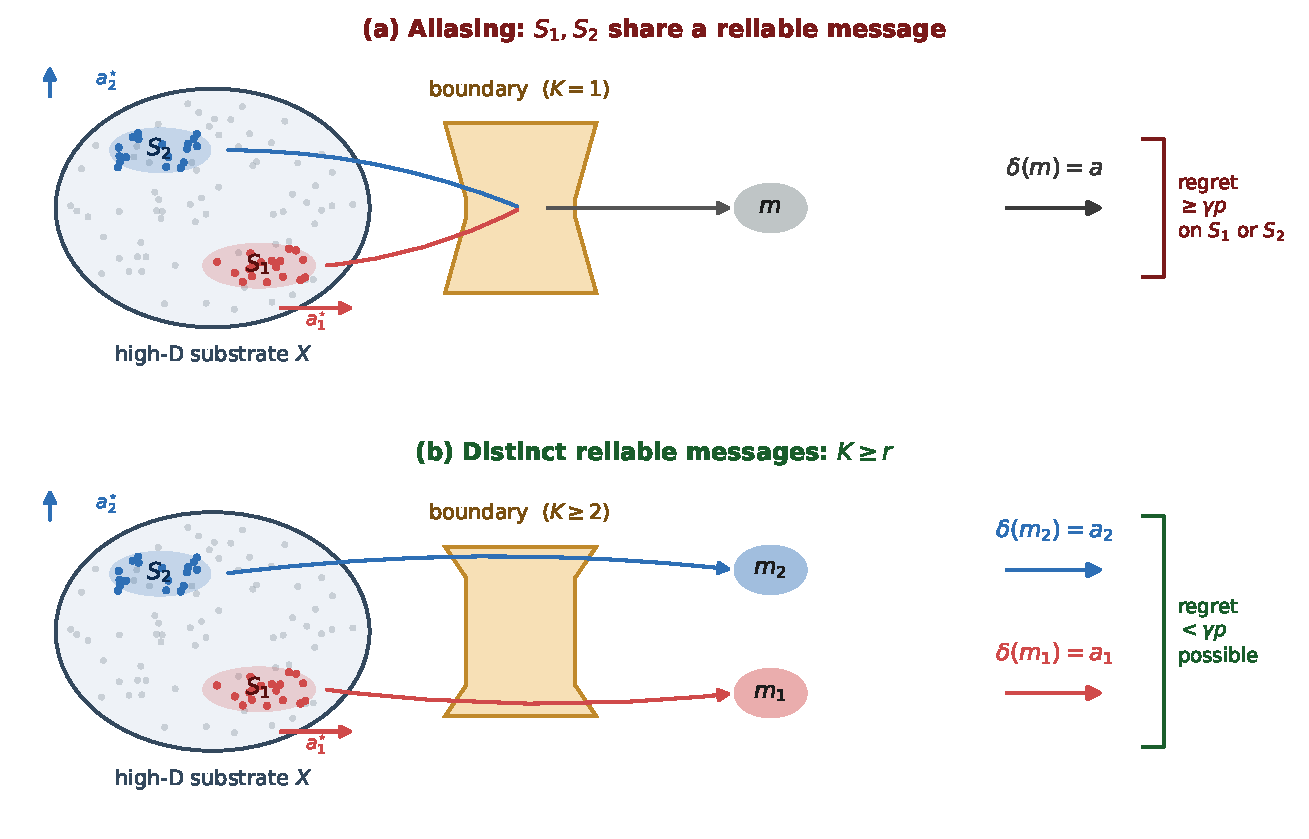
\includegraphics[width=\textwidth]{figures/fig1_boundary_code_schematic.pdf}
\caption{Schematic of forced codeword separation. Two recurrent substrate regimes, $S_1$ and $S_2$, require mutually incompatible responses. If a one-message boundary aliases both regimes to the same reliable message, the decoder must choose a single action and incurs regret at least $\gamma p$ on at least one regime. A low-regret protocol must therefore allocate distinct reliable messages to the incompatible regimes; for $r$ such regimes this requires at least $\log_2 r$ reliable bits. Distinct messages make regret below $\gamma p$ possible, subject to a decoder that assigns each message a good action.}
\label{fig:boundary-code}
\end{figure}

\section{The boundary-code principle}
\label{sec:theorem}

\subsection{Projection insufficiency}

\begin{lemma}[Projection insufficiency]
\label{lem:projection}
Let $Z=g(X)$ be the task-relevant variable for a coordination task with substrate distribution $P_X$, and let $d_Z$ be the distortion induced on $Z$ by the coordination loss. If the rate-distortion function $R_Z(D^\star)$ for $Z$ at expected distortion $D^\star$ exceeds the boundary budget $\C T$, then no boundary channel of capacity $\C$ over duration $T$ can support coordination at expected distortion no greater than $D^\star$.
\end{lemma}

\begin{proof}
By the converse of rate-distortion theory, any representation of $Z$ achieving expected distortion no greater than $D^\star$ requires rate at least $R_Z(D^\star)$ \citep{coverthomas2006}; the boundary channel supplies at most $\C T$ bits.
\end{proof}

If the substrate's task-relevant state exceeds boundary capacity, direct state sharing is impossible. The system must either fail, increase capacity, change the task, or compress.

\subsection{Non-recoverability}

\begin{lemma}[Non-recoverability after projection]
\label{lem:nonrecoverability}
For any deterministic or stochastic downstream computation $Y=f(M)$ and any variable $U$ inducing the Markov chain $U \to X \to M \to Y$, the data-processing inequality gives
\[
\I(U;Y) \leq \I(U;M).
\]
Distinctions in $U$ that the projection has discarded cannot be recovered from $M$ alone, absent side information or an entrained receiver context (see Proposition~\ref{prop:latent} for the case in which receiver context partially compensates).
\end{lemma}

\begin{proof}
Direct application of the data-processing inequality \citep{coverthomas2006}.
\end{proof}

The downstream system can sample or reconstruct likely substrate states from the message, but it cannot recover the actual distinctions erased by the projection. Code formation must therefore act on the projection itself.

\subsection{Cascade non-increase along radial boundaries}
\label{sec:cascade}

The collapse argument so far treats the boundary as a single sharp interface. The same conclusion holds, with the same proof, for the radial idealization in which the substrate, channel, and receiver are connected by a longer Markov cascade. The next lemma states this precisely; it is the formal foundation of the volumetric picture invoked in the framework remark of Section~\ref{sec:framework} and instantiated empirically in Section~\ref{sec:emergence}.

\begin{lemma}[Cascade non-increase]
\label{lem:cascade}
Let $U$ be any finite-entropy task-relevant variable measurable with respect to $X$, and let
\[
X = Z_0 \to Z_1 \to \cdots \to Z_L \to M \to W_1 \to \cdots \to W_J \to A
\]
form a Markov cascade with discrete waist alphabet $|\M|\leq K$ and reliable-message budget $\I(Z_L;M)\leq \C T$. Then
\begin{align*}
\I(U;Z_{i+1}) &\;\leq\; \I(U;Z_i) && \text{for } 0\leq i<L, \\
\I(U;M) &\;\leq\; \min\!\big\{\I(U;Z_L),\;\log_2 K,\;\C T\big\}, \\
\I(U;W_j) &\;\leq\; \I(U;M) && \text{for all } 1\leq j\leq J, \\
\I(U;W_{j+1}) &\;\leq\; \I(U;W_j) && \text{for } 1\leq j<J.
\end{align*}
\end{lemma}

\begin{proof}
Each inequality is an instance of the data-processing inequality \citep{coverthomas2006} applied to the appropriate sub-chain. The bound $\I(U;M)\leq\log_2 K$ is the entropy bound on a discrete random variable of cardinality at most $K$; the bound $\I(U;M)\leq\C T$ is the boundary-channel budget of Definition~\ref{def:boundarychannel}.
\end{proof}

The conclusion is geometric. Decoder-side re-expansion may increase covariance rank, embedding dimension, or the participation-ratio measure of $D_{\rm eff}$ used in the simulations, but it cannot recover task-relevant distinctions about $U$ that were absent from $M$. ``Boundary'' is therefore better thought of as the depth at which $\I(U;Z_i)$ first falls to the rate-distortion floor implied by Lemma~\ref{lem:projection} than as a single mathematical surface; everything past that depth is downstream of an irreversible projection.

\subsection{Stable partitions}

\begin{proposition}[Fiber coherence from low expected regret]
\label{prop:partition}
For a finite boundary protocol $(\pi,\delta)$, $\pi$ induces a finite partition of $\X$ into message fibers $\pi^{-1}(m)$. If the protocol achieves expected regret at most $\eps$, then for every $\eta\in(0,1]$ there is an exception set $E_\eta$ of probability at most $\eta$ such that for every $x\notin E_\eta$ the regret under the assigned response $\delta(\pi(x))$ is at most $\eps/\eta$. Restricted to $\X\setminus E_\eta$, every occupied fiber is therefore $\eps/\eta$-coherent under its assigned response.
\end{proposition}

\begin{proof}
Let $r(x)=\loss(x,\delta(\pi(x)))-\loss^\star(x)\geq 0$. By assumption $\E[r(X)]\leq\eps$, so by Markov's inequality $P\{r(X)>\eps/\eta\}\leq\eta$. Set $E_\eta=\{x:r(x)>\eps/\eta\}$.
\end{proof}

A useful codeword is not an arbitrary bin: it is a fiber whose assigned response is near-optimal across almost all of its mass.

\begin{proposition}[Boundary-code structure of retained low-loss protocols]
\label{prop:boundarycode}
Consider a recurrent coordination problem between a high-dimensional substrate $X$ and a downstream system across a boundary channel of capacity $\C$. Assume:
\begin{enumerate}
\item the task-relevant information in $X$ exceeds the boundary budget for direct state transmission;
\item coordination episodes recur under a stationary or slowly varying distribution $P_X$;
\item boundary protocols vary by mutation, learning, plasticity, development, or selection;
\item protocol variants with lower expected loss are preferentially retained;
\item the channel alphabet is finite or effectively finite over each coordination episode.
\end{enumerate}
Then any retained protocol whose expected regret is at most $\eps$ (``low-loss'') takes the form of a finite partition of $\X$ whose occupied fibers, away from a small exception set, are coherent under their assigned responses in the sense of Proposition~\ref{prop:partition}. If the partition is reused across episodes and interpreted by downstream dynamics, the protocol is a biological code. This is a structural characterization of low-loss retained protocols; an explicit alternating-improvement dynamics whose limit points realize this structure is given in Section~\ref{sec:convergence}.
\end{proposition}

\begin{proof}
By Lemma~\ref{lem:projection}, direct transmission of the task-relevant substrate state is impossible. Any successful protocol must therefore compress $X$ into messages $M$ whose cardinality or mutual information is bounded by the channel; such an encoder $\pi$ induces a finite partition of $\X$ into fibers. By Lemma~\ref{lem:nonrecoverability}, distinctions discarded by $\pi$ cannot be recovered downstream, so selection on coordination success can only improve performance by changing the partition, the decoder, the channel, or the substrate distribution. Under a fixed boundary and recurrent task distribution, a retained low-loss protocol cannot group high-probability incompatible states into a common fiber, since this forces the assigned response to be far from optimal for one or both. Proposition~\ref{prop:partition} then implies that, away from a small exception set, every occupied fiber is coherent under its assigned response. Recurrence makes the partition reusable; downstream response implements interpretation; preferential retention supplies viability coupling.
\end{proof}

The proposition does not say that every retained protocol is globally optimal. Biological evolution and learning find local optima, path-dependent conventions, and historically frozen mappings. The claim is that whatever low-loss mapping is retained at such a boundary has the structure of a finite action-relevant partition.

\begin{corollary}[Code cardinality]
\label{cor:cardinality}
$\I(X;M)\leq \C T$. In the noiseless case, $|\M|\leq 2^{\C T}$. With noise, separation margins and error-control overhead reduce the usable alphabet below the noiseless count.
\end{corollary}

\begin{corollary}[No-code regime]
\label{cor:nocode}
If the boundary channel can transmit the task-relevant substrate dynamics at the required distortion, continuous coupling can solve the coordination problem without a finite code. Codes are expected at boundaries where direct coupling fails, not inside regimes of preserved timing and state access.
\end{corollary}

\begin{corollary}[Shadow complexity]
\label{cor:shadow}
The complexity discarded by a code remains in the fibers as within-codeword variation. Higher-bandwidth observers may resolve structure invisible at the code layer.
\end{corollary}

\subsection{Convergence by alternating improvement}
\label{sec:convergence}

Proposition~\ref{prop:boundarycode} characterizes the form of retained low-loss protocols but does not by itself describe a dynamics that reaches them. The following two results give an explicit alternating-improvement dynamics --- finite-bandwidth viability optimization read as a generalized Lloyd--Bayes iteration --- whose risk decreases monotonically and whose limit points are partition-shaped.

\begin{proposition}[Voronoi--Bayes coordinatewise optimality]
\label{prop:voronoibayes}
Let $\M$ be a finite alphabet, $\A$ a compact action set, $\ell$ a continuous viability loss with $\sup_{x,a}\ell(x,a) < \infty$ on the support of $P_X$ (or $\ell$ integrable under $P_X$ for every fixed $a$), and $P_X$ a substrate distribution.
\begin{enumerate}
\item For any decoder $\delta:\M\to\A$, the encoder minimizing $L(\pi,\delta)=\E[\ell(X,\delta(\pi(X)))]$ is the loss-Voronoi assignment
\[
\pi^\star(x) \in \arg\min_{m\in\M}\,\ell(x,\delta(m)),
\]
under arbitrary deterministic tie-breaking on the tie set $\{x:|\arg\min_m\ell(x,\delta(m))|>1\}$, and unique when that tie set has $P_X$-measure zero.
\item For any encoder $\pi$ inducing cells $F_m=\pi^{-1}(m)$ of positive probability, the decoder minimizing $L(\pi,\delta)$ is the Bayes action per cell,
\[
\delta^\star(m) \in \arg\min_{a\in\A}\,\E\!\left[\ell(X,a)\,\big|\,X\in F_m\right].
\]
\end{enumerate}
\end{proposition}

\begin{proof}
Pointwise minimization. For (1), and any $\delta$,
\[
L(\pi,\delta)=\E[\ell(X,\delta(\pi(X)))]\;\geq\;\E[\min_m \ell(X,\delta(m))],
\]
with equality when $\pi$ assigns each $x$ to a minimizer; the minimizer is unique off the tie set. For (2), on each cell $F_m$, $\E[\ell(X,\delta(m))\mid X\in F_m]$ is minimized by the Bayes action by definition.
\end{proof}

\begin{proposition}[Lloyd--Bayes monotone improvement]
\label{prop:lloydbayes}
Fix a deterministic tie-breaking rule for the encoder step, a fixed Bayes-action selector for the decoder step, and a fixed empty-cell handling rule. Define the alternating Lloyd--Bayes update: at each step, hold one of $(\pi,\delta)$ fixed and replace the other by its risk-minimizer per Proposition~\ref{prop:voronoibayes}. Then the expected risk $L^{(k)}=L(\pi^{(k)},\delta^{(k)})$ is non-increasing in $k$. Since $L^{(k)}\geq 0$, the risk sequence converges. For finite or discretized $P_X$, under the standard no-cycling/tie-handling convention for generalized Lloyd iteration, the iteration reaches a coordinatewise stationary protocol --- one satisfying both fixed-point conditions of Proposition~\ref{prop:voronoibayes} --- in finitely many steps \citep{linde1980,gray1998}.
\end{proposition}

\begin{proof}
Each Lloyd--Bayes step replaces one factor of $(\pi,\delta)$ by a coordinatewise risk-minimizer (Proposition~\ref{prop:voronoibayes}), so $L^{(k+1)}\leq L^{(k)}$. The monotone bounded sequence $L^{(k)}$ converges. For finite/discretized $P_X$ under the no-cycling/tie-handling convention, the trajectory lies in a finite set of partition--decoder pairs and the iteration enters a coordinatewise stationary configuration in finitely many steps.
\end{proof}

We do \emph{not} claim convergence of $(\pi^{(k)},\delta^{(k)})$ for continuous $P_X$; that requires further regularity assumptions and is treated in the quantization-theory literature \citep{linde1980,gray1998,sabin1986}.

\begin{corollary}[Idealized code-formation mechanism]
\label{cor:codeformation}
Finite-bandwidth viability optimization has partition-shaped fixed points. When biological selection, learning, plasticity, or development can be approximated by an alternating improvement dynamic on encoder and decoder --- selection or plasticity refining within-fiber action choice given the current partition; mutation, learning, or developmental variation refining the partition given the current action repertoire --- the resulting protocol is expected to approach such a fixed point. Coherence of the reached protocol's fibers in the sense of Definition~\ref{def:fiber} is a separate claim, supplied by Proposition~\ref{prop:partition} from the achieved expected regret: the lower the rate-distortion floor of Lemma~\ref{lem:projection} permits the risk to fall, the tighter the resulting fiber coherence.
\end{corollary}

This is an idealized mechanism, not the claim that biology runs Lloyd--Bayes literally. The point is that Proposition~\ref{prop:boundarycode}'s structural characterization is realized by a standard alternating-improvement dynamics: under finite-bandwidth viability optimization, codes are not just the form of retained low-loss protocols; they are the fixed points of an explicit improvement procedure, reached by exact alternating updates in the finite/discretized case, up to local optima and tie-handling. The selection-driven emergence in Section~\ref{sec:emergence} is approximately such a dynamics with mutation noise as the search operator.

\subsection{Forced nontrivial codes}
\label{sec:forced}

Existence and reachability (Propositions~\ref{prop:voronoibayes}--\ref{prop:lloydbayes}) say that partition stationary points form, but do not by themselves say the partition must be nontrivial: a degenerate one-codeword partition is also a fixed point. The next result fills that gap. When the substrate contains mutually action-incompatible regimes, any low-regret protocol is forced to allocate distinct codewords to them, or pay an explicit regret floor.

\begin{definition}[$\gamma$-bad action; pointwise $\gamma$-action-incompatibility]
\label{def:incompatible}
An action $a \in \A$ is \emph{$\gamma$-bad on a region} $S \subseteq \X$ when $\ell(x,a) - \ell^\star(x) \geq \gamma$ for $P_X$-almost every $x \in S$. Two regions $S, S'$ of positive $P_X$-mass are \emph{pointwise $\gamma$-action-incompatible} when every action $a \in \A$ is $\gamma$-bad on at least one of $S, S'$. A family $\{S_1, \ldots, S_r\}$ is \emph{mutually pointwise $\gamma$-action-incompatible} when every pair is.
\end{definition}

Pointwise incompatibility is a sufficient condition for the result below, not a necessary one --- pairs of regions can fail to satisfy it and codes can still form --- but it is the cleanest setting in which forced separation can be proved.

\begin{proposition}[Forced nontrivial code]
\label{prop:forced}
Let $S_1, \ldots, S_r$ be mutually pointwise $\gamma$-action-incompatible regions with $\min_i P_X(S_i) \geq p > 0$, and let $(\pi, \delta)$ be any boundary protocol.
\begin{enumerate}
\item If the expected regret satisfies $L(\pi,\delta) - L^\star < \gamma p$, then $\pi$ uses at least $r$ distinct messages on the support of $\bigcup_i S_i$, and the boundary alphabet must satisfy $|\M| \geq r$ (equivalently, at least $\log_2 r$ reliably distinguishable messages).
\item Conversely, if the boundary alphabet has fewer than $r$ reliably distinguishable messages, the expected regret is bounded below by $\gamma p$: at least one action-incompatible regime must alias, and the system pays the corresponding viability cost.
\end{enumerate}
\end{proposition}

\begin{proof}
For each $i$, define the set of messages whose decoded action is \emph{not} $\gamma$-bad on $S_i$,
\[
G_i \;=\; \{\,m \in \M : \delta(m) \text{ is not } \gamma\text{-bad on } S_i\,\}.
\]
By pointwise $\gamma$-action-incompatibility, every action is $\gamma$-bad on at least one of any two regions, so for $i \neq j$ no action can fail to be $\gamma$-bad on both. Hence $G_i \cap G_j = \emptyset$.

For each $i$, the contribution to expected regret from states in $S_i$ assigned to messages outside $G_i$ is bounded below pointwise by $\gamma$:
\[
L(\pi,\delta) - L^\star \;\geq\; \E\!\big[(\ell(X,\delta(\pi(X))) - \ell^\star(X))\,\mathbf{1}_{X\in S_i,\;\pi(X)\notin G_i}\big] \;\geq\; \gamma \cdot P\!\big(X\in S_i,\,\pi(X)\notin G_i\big).
\]
Rearranging,
\[
P\!\big(X\in S_i,\,\pi(X)\in G_i\big) \;\geq\; P_X(S_i) - \frac{L(\pi,\delta) - L^\star}{\gamma}.
\]

\emph{Part (1).} If $L(\pi,\delta) - L^\star < \gamma p$, the right-hand side is strictly positive ($> P_X(S_i) - p \geq 0$). So for each $i$ there is at least one message in $G_i$ used by $\pi$ on positive mass of $S_i$. By disjointness of the $G_i$, the chosen messages are pairwise distinct, giving at least $r$ distinct used messages and hence $|\M| \geq r$.

\emph{Part (2).} If fewer than $r$ messages are reliably distinguishable, the disjoint sets $G_1,\ldots,G_r$ cannot all be nonempty: at least one $G_i$ must be empty. For that $S_i$, every used message has decoded action $\gamma$-bad on $S_i$, so $\ell(x,\delta(\pi(x))) - \ell^\star(x) \geq \gamma$ for $P_X$-a.e.\ $x \in S_i$, giving $L(\pi,\delta) - L^\star \geq \gamma P_X(S_i) \geq \gamma p$.
\end{proof}

The conclusion requires no decisiveness or majority condition on the encoder. It uses only the Markov-style fact that low expected regret forces most of each region's mass to its good-message set, and the disjointness of those sets follows from incompatibility alone.

\paragraph{Combined claim.} Propositions~\ref{prop:boundarycode}, \ref{prop:lloydbayes}, and \ref{prop:forced} together give the substantive code-formation result of this paper:
\begin{itemize}
\setlength\itemsep{0pt}
\item finite-bandwidth viability optimization has partition fixed points (Proposition~\ref{prop:boundarycode});
\item alternating Lloyd--Bayes improvement reaches such fixed points in the finite/discretized case, up to local optima and tie-handling (Proposition~\ref{prop:lloydbayes});
\item when the substrate contains $r$ mutually action-incompatible regimes of mass $\geq p$, any protocol with regret below $\gamma p$ is forced to allocate distinct codewords to them, and below the corresponding capacity the regret floor $\gamma p$ acts (Proposition~\ref{prop:forced}).
\end{itemize}
Codes form, and under the stated conditions they are nontrivial.

\subsection{Anticipation by synchronization}

\begin{proposition}[Trajectory-preserving codes carry predictive information]
\label{prop:anticipation}
Let the trajectory coordinate $\phi_t$ of a slow mode drive both substrate and future. Assume the directed graphical model
\[
\phi_t \to X_t \to M_t,\qquad \phi_t \to F_{t+\Delta},\qquad 0<\Delta<\tau_W,
\]
with $M_t=\pi(X_t)$ and $F_{t+\Delta}\perp X_t,M_t\mid\phi_t$. Let $Q=q(\phi_t)$ be a finite trajectory partition that is a sufficient statistic for predicting the future variable from $\phi_t$, so that
\[
M_t \perp F_{t+\Delta}\mid Q.
\]
($Q$ is not generated from $M_t$; it is an external summary of $\phi_t$, and the conditional independence captures sufficiency.) Then
\[
\I(M_t;F_{t+\Delta}) \;\geq\; \I(M_t;Q) - H(Q\mid F_{t+\Delta}).
\]
The right-hand side is positive whenever the message resolves $Q$ better than the future does. In the deterministic case $F_{t+\Delta}=h(Q)$ with $h$ injective on the support of $Q$, $H(Q\mid F_{t+\Delta})=0$ and the bound becomes equality, $\I(M_t;F_{t+\Delta})=\I(M_t;Q)$.
\end{proposition}

\begin{proof}
The conditional independences $F_{t+\Delta}\perp X_t\mid\phi_t$ and $F_{t+\Delta}\perp\phi_t\mid Q$ imply $F_{t+\Delta}\perp M_t\mid Q$, so $\I(M_t;F_{t+\Delta}\mid Q)=0$. The chain rule then gives $\I(M_t;F_{t+\Delta})=\I(M_t;Q)-\I(M_t;Q\mid F_{t+\Delta})\geq\I(M_t;Q)-H(Q\mid F_{t+\Delta})$. When $F_{t+\Delta}=h(Q)$ is deterministic and $h$ is injective on the support of $Q$, $Q$ is recoverable from $F_{t+\Delta}$, so $\I(M_t;Q\mid F_{t+\Delta})=0$ and the bound becomes equality.
\end{proof}

The trajectory coordinate is the common driver of substrate and future, not a child of substrate. Boundary messages inherit predictive content because the encoder is sensitive to substrate variation that is itself driven by the slow mode.

\begin{corollary}[Anticipation by synchronization]
\label{cor:syncanticipation}
A substrate entrained to a slow mode can behave anticipatorily without explicitly representing future microstates. The anticipatory horizon is bounded by the coherence time of the longest task-relevant slow mode preserved by the code.
\end{corollary}

This is the bridge between code formation and biological intelligence. Fast local dynamics supply flexibility; slow-mode synchronization supplies horizon. Circadian systems prepare metabolism before dawn not because they simulate sunrise from first principles each night, but because the organism is entrained to the day--night cycle.

\subsection{Latent context: code--context as the operational unit}
\label{sec:latent}

Proposition~\ref{prop:anticipation} locates anticipatory information in the boundary message itself. In biology the predictive content often resides instead in the receiver's entrained internal state: the same hormone pulse means different things at different circadian phases, the same morphogen at different developmental stages, the same spike burst at different oscillatory phases, the same antigen signal during repair, infection, or prior exposure.

\begin{proposition}[Latent anticipation through context]
\label{prop:latent}
Suppose the receiver carries a phase-conditioned context $C_t=c(\phi_t)$ and acts via $A_t=\delta(M_t,C_t)$. Under the directed model of Proposition~\ref{prop:anticipation},
\[
\I((M_t,C_t);F_{t+\Delta}) \;\geq\; \I(C_t;F_{t+\Delta}),
\]
which is positive whenever $C_t$ preserves a class of $\phi_t$ distinguishing the future-conditional distribution. The receiver therefore has access to anticipatory information through context alone, even in the limit $\I(M_t;\phi_t)=0$.
\end{proposition}

\begin{proof}
The chain rule gives $\I((M_t,C_t);F_{t+\Delta})=\I(C_t;F_{t+\Delta})+\I(M_t;F_{t+\Delta}\mid C_t)\geq\I(C_t;F_{t+\Delta})$. Applying Proposition~\ref{prop:anticipation} with $C_t$ in place of $M_t$ gives $\I(C_t;F_{t+\Delta})>0$ whenever $C_t$ preserves a sufficient $Q$-class.
\end{proof}

Whether the available anticipation is realized in action is a separate question about $\delta$: by the data-processing inequality $\I(A_t;F_{t+\Delta})\leq\I((M_t,C_t);F_{t+\Delta})$, with equality when $\delta$ maps future-relevant context classes to distinguishable actions. Proposition~\ref{prop:latent} bounds the information available to the receiver; realization in $A_t$ depends on the decoder using it. The effective codeword is often the pair $(M_t,C_t)$, not $M_t$ alone, so an external observer reading only the boundary message may underestimate predictive content correspondingly.

\begin{corollary}[Observer-hidden anticipatory context]
\label{cor:hidden}
For any observer-accessible readout $O_t=r(M_t,C_t)$,
\[
\I((M_t,C_t);F_{t+\Delta}) \;\geq\; \I(O_t;F_{t+\Delta}),
\]
with strict inequality possible whenever $r$ discards future-relevant context. Null measurements of predictive content in transmitted codewords are therefore weak evidence against anticipation. The relevant test is whether \emph{behavior} retains its future-conditional structure under interventions on slow modes, not whether the boundary signal visibly carries phase.
\end{corollary}

The receiver has access to $C_t$ \emph{by being} $C_t$; the observer accesses it only through a measurement channel of finite capacity. This is the same observer--substrate asymmetry that drives the falsifiability and timing-inaccessibility results in the prior papers \citep{todd2025falsifiability,todd2025maxwell}.

\paragraph{Slow modes as changes in meaning.} Over short windows, a slow mode looks like a constant background and contributes little to instantaneous variation. Its causal force becomes visible at \emph{gating events} --- phase transitions, competence windows, threshold crossings --- at which $C_t$ moves into a regime where the same boundary message is interpreted differently:
\begin{itemize}
\item Local hormonal and metabolic signals look similar moment to moment; their consequences flip at sleep--wake, feeding--fasting, and immune-tone gates.
\item Cells can carry similar molecular markers across a stage boundary; the same morphogen is permissive before commitment and instructive after.
\item A spike or burst can look locally similar; its postsynaptic and behavioral impact depends on theta/beta/gamma phase gates.
\item The same antigen presentation is interpreted differently across infection stage, repair stage, prior priming, exhaustion, or tolerance.
\item A gesture or phrase can be lexically stable; its meaning shifts at relational, ritual, or commitment boundaries.
\end{itemize}
Strong biological codes preserve access to slow-mode context, either by encoding it in the message or by coupling the decoder to an entrained context that changes how the same message is interpreted.

\begin{proposition}[Slow-mode boundary-code principle]
\label{prop:longwave}
Consider a recurrent coordination problem in which future loss depends on a coherent slow mode and (with positive probability under $P_X$) different trajectory classes of that mode admit no shared near-optimal response across the future horizon. Then retained low-loss code--context systems must preserve those distinctions whose merger would exceed the tolerated regret, subject to boundary capacity. The required slow-trajectory information is carried by the message, by the receiver's entrained context, or by a combination of the two.
\end{proposition}

\begin{proof}
By Proposition~\ref{prop:boundarycode}, retained low-loss codes have fibers approximately coherent under their assigned responses. The added assumption says that with positive probability two substrate states from distinct trajectory classes cannot share a single near-optimal response over the future horizon; merging them into a common fiber therefore incurs nonzero expected regret, which is incompatible with retention. The system must distinguish the trajectory classes at decision time. Propositions~\ref{prop:anticipation} and \ref{prop:latent} establish two routes for doing so: trajectory-preserving messages and phase-conditioned context, respectively.
\end{proof}

\subsection{Worked example: one-bit slow-mode code}

A minimal numerical example shows what the slow-mode claim adds beyond generic compression. Let
\[
X_t=(\cos\phi_t,\sin\phi_t)+\eta_t,
\]
with $\eta_t$ Gaussian noise and $\phi_t$ a coherent slow phase. The boundary transmits one bit, and the loss depends on a future binary task variable $F_{t+\Delta}=\mathbf{1}\{\cos(\phi_t+\Delta)>0\}$. A phase-blind present-axis code $M=\mathbf{1}\{X_1>0\}$ has one bit but preserves the wrong distinction at any nontrivial $\Delta$. A search over one-bit linear partitions $M_\theta=\mathbf{1}\{\cos\theta\,X_1+\sin\theta\,X_2>0\}$ finds the loss-minimizing projection. Figure~\ref{fig:phase-demo} reports the result: at $\Delta=\pi/2$ the present-axis cut is at chance accuracy ($0.50$), the best one-bit cut reaches $0.88$, and the oracle reaches $1.00$. Sweeping $\Delta$ over $[0,\pi]$, the best one-bit accuracy stays near $0.88$ across the whole sweep while the present-axis accuracy varies sinusoidally; the recovered projection-vector angle tracks the theoretical optimum $-\Delta$ throughout. Under a one-bit boundary, the useful codeword is the partition that preserves the future-relevant slow-mode class, not the partition that best labels an arbitrary present coordinate.

\begin{figure}[H]
\centering
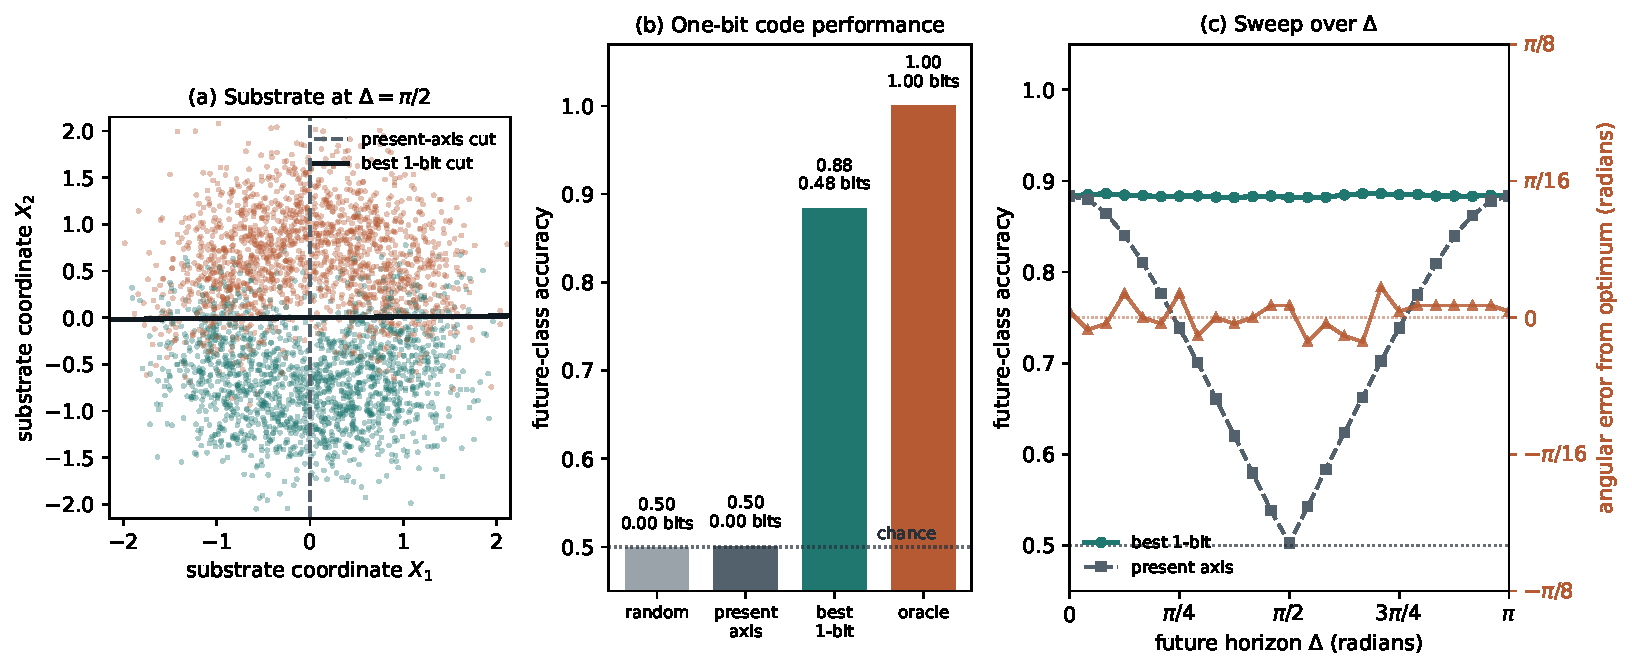
\includegraphics[width=\textwidth]{figures/fig2_phase_partition_demo.pdf}
\caption{The useful one-bit code preserves the future-relevant slow-mode class, not an arbitrary present coordinate. Substrate $X_t=(\cos\phi_t,\sin\phi_t)+\eta_t$ with $\sigma=0.42$ and $n=120{,}000$; in panels (a, c) colour encodes the future class $F_{t+\Delta}$. (a) Substrate at $\Delta=\pi/2$ with present-axis cut (dashed) and future-relevant cut (solid). (b) Accuracy and mutual information at $\Delta=\pi/2$ for random, present-axis, future-relevant, and oracle codes. (c) Sweep over $\Delta\in[0,\pi]$: the future-relevant 1-bit code stays high while the present-axis code varies sinusoidally between perfect and chance. The recovered projection angle tracks the theoretical optimum $-\Delta$ (modulo the partition's $\pi$-periodicity) across the sweep; numerical recovery details are in \texttt{figures/phase\_partition\_results.txt}. Reproducible code in \texttt{simulations/generate\_figures.py}.}
\label{fig:phase-demo}
\end{figure}

\section{Conditional universality for bounded self-maintaining systems}
\label{sec:universal}

Proposition~\ref{prop:forced} is conditional. The empirical claim that living systems form codes is universal. The gap is closed by axiomatizing bounded self-maintenance and showing the axioms imply the conditions of Proposition~\ref{prop:forced}. The axioms below are not invented to yield codes; they aggregate standard commitments of autopoiesis \citep{maturana1980,polanyi1968}, Schr\"odinger--Prigogine non-equilibrium thermodynamics \citep{schrodinger1944,prigogine1977}, complexity theory, life-history theory, and selection theory. Codes are derived.

\subsection{Axioms}

\begin{axiom}[Autopoietic boundary closure]
\label{ax:closure}
A living system maintains a boundary $\partial$ distinguishing interior $\Omega$ from environment, self-produced and self-maintained by interior dynamics; dissolution of $\partial$ entails dissolution of the system.
\end{axiom}

\begin{axiom}[Non-equilibrium maintenance]
\label{ax:nonequilibrium}
The interior $\Omega$ persists only by exchanging matter, energy, or information across $\partial$ at rates sufficient to maintain organization away from thermodynamic equilibrium. Cessation of such exchange entails relaxation toward equilibrium.
\end{axiom}

\begin{axiom}[Finite boundary throughput]
\label{ax:finite}
The boundary $\partial$ has finite reliable throughput in the sense of Definition~\ref{def:boundarychannel}.
\end{axiom}

\begin{axiom}[High-dimensional interior]
\label{ax:highd}
The interior state $\Omega$ has effective dimension exceeding the boundary's reliable capacity over the relevant coordination timescales.
\end{axiom}

\begin{axiom}[Action-incompatible regimes]
\label{ax:incompat}
The interior dynamics admit at least two recurrent regimes $S_1, S_2 \subseteq \Omega$ of positive measure on persistence timescales, mutually pointwise $\gamma$-action-incompatible (Definition~\ref{def:incompatible}) for some $\gamma > 0$, with dissolution a positive-probability outcome of incorrect response selection.
\end{axiom}

This is the substantive condition. Non-equilibrium maintenance plus a non-trivial life cycle motivates it: replication, repair, defense, and growth phases are not interchangeable in their action requirements, and an organism cycling between them faces regimes whose optimal responses differ. The negative case is loss of maintained heterogeneity --- whether environmental, internally generated, or both --- which removes the action-incompatible regimes and triggers the no-code regime of Corollary~\ref{cor:nocode}. External homogeneity by itself is not the killer: a living system can sit in a uniform bath while maintaining internal cycling. What excludes the no-code regime for living systems is the persistence of maintained heterogeneity that Axiom~\ref{ax:nonequilibrium} requires. The theorem requires Axiom~\ref{ax:incompat} explicitly; the connection to Axiom~\ref{ax:nonequilibrium} is motivation, not derivation.

\begin{axiom}[Retention]
\label{ax:retention}
Mappings from interior state to boundary action that reduce expected viability loss are preferentially stabilized by selection, learning, plasticity, development, or homeostasis.
\end{axiom}

\subsection{Theorem}

\begin{proposition}[Conditional universality of nontrivial codes]
\label{prop:universal}
Any system satisfying Axioms~\ref{ax:closure}--\ref{ax:retention} forms at least one nontrivial code at at least one of its boundaries: any low-regret protocol it maintains across that boundary uses at least two distinct reliable codewords, or pays a regret floor incompatible with persistence on the relevant timescale.
\end{proposition}

\begin{proof}
Axioms~\ref{ax:closure}, \ref{ax:finite}, \ref{ax:highd}, \ref{ax:incompat} supply the hypotheses of Proposition~\ref{prop:forced} with $r=2$: a self-produced boundary $\partial$ with finite reliable throughput, a high-dimensional interior, and two pointwise $\gamma$-action-incompatible regimes $S_1, S_2$ of mass $\geq p$. Axiom~\ref{ax:nonequilibrium} supplies their recurrence on persistence timescales; Axiom~\ref{ax:retention} supplies viability-coupled retention of low-regret protocols. By Proposition~\ref{prop:forced}, any retained protocol either uses at least two distinct reliable codewords across $S_1 \cup S_2$, or its expected regret is bounded below by $\gamma p$. The latter is incompatible with persistence by the dissolution clause of Axiom~\ref{ax:incompat}, so the retained protocol must use at least two distinct reliable codewords.
\end{proof}

The conclusion is the minimal result: at least two codewords. Real biological systems satisfy the conditions for $r \gg 2$ --- codons, spike alphabets, cell-fate alphabets, immune repertoires --- because the action-incompatibility number of an organized living substrate is large; the proposition only guarantees the floor.

\subsection{Status of the universality claim}

The axioms do not mention codes, partitions, or messages. They describe boundary closure, non-equilibrium maintenance, finite throughput, multi-component interior, action-incompatible regimes, and retention --- each operationally specifiable without reference to coding. The package is over-determined: each axiom has independent provenance in a separate intellectual tradition (autopoiesis, non-equilibrium thermodynamics, complexity theory, life-history theory, selection theory), and rejecting any single tradition leaves the others standing. The result is therefore not ``biology forms codes because we have defined biology as code-forming,'' but ``codes follow from a small set of commitments standardly held about life, none of which were assembled to yield codes.''

\begin{corollary}[Conditional universality of biological codes]
\label{cor:calibrated}
Within the axiomatic framework of Axioms~\ref{ax:closure}--\ref{ax:retention}, any system satisfying the axioms forms at least one nontrivial code at at least one of its boundaries. Insofar as the axioms accurately characterize living organization --- as five independent biological traditions assert they do --- every living system forms at least one nontrivial code.
\end{corollary}

The corollary does not derive any particular alphabet, does not claim global optimality of any reached code, and does not extend to systems violating an axiom --- in particular, systems out of non-equilibrium maintenance on the relevant timescale (dormant spores under sufficient quiescence) fall outside Axiom~\ref{ax:nonequilibrium} and are not bound by the theorem until they re-enter active maintenance.

\section{Code formation in simulation: emergence, volumetric structure, and the cardinality floor}
\label{sec:emergence}

Section~\ref{sec:convergence} gives an idealized alternating-improvement mechanism for which partition-shaped fixed points exist. Real biological selection, learning, and plasticity are not literal Lloyd--Bayes iteration; nor are real biological boundaries sharp two-zone interfaces. This section reports three numerical experiments that, taken together, instantiate the boundary-code principle in increasingly realistic settings: (i)~a one-channel selection-driven emergence demonstration; (ii)~a multi-layer hourglass simulator with a continuous radial dimensionality profile and a single discrete waist, sweeping the waist alphabet to verify the cardinality floor of Proposition~\ref{prop:forced}; and (iii)~a slow-mode preservation test that confirms the predicted dissociation between fast and slow modes through the waist.

\subsection{Selection finds the partition}

The substrate is six-dimensional: the first two coordinates carry the slow-mode signal $(\cos\phi_t,\sin\phi_t)+\eta_t$, the remaining four are Gaussian distractor noise the encoder must learn to ignore. The boundary carries two bits ($K=4$ codewords). The future task is the four-class label of $\phi_t+\pi/2$. An encoder $\pi_\theta$ chooses a codeword as the argmax of $K$ linear projections of $X$; a decoder $\delta\in\{0,\ldots,K-1\}^K$ is a lookup table from codeword to predicted class. A population of $64$ pairs evolves for $250$ generations under top-half selection on future-class accuracy. A drift control runs the same mutation operator with parents drawn uniformly at random.

A random individual at generation $0$ produces a speckled partition near chance ($1/4$). After $250$ generations of selection, the best individual carries a clean four-quadrant partition aligned with the slow-mode-determined future classes; the drift control wanders without converging on the slow-mode-relevant subspace. Selection drives accuracy from near-chance to roughly $0.75$ within the first $50$ generations and stabilizes there; the drift control fluctuates around $0.4$. The channel capacity and the action set are fixed by construction, but the substrate partition and the codeword-to-action mapping are not pre-specified; selection finds them.

\begin{figure}[H]
\centering
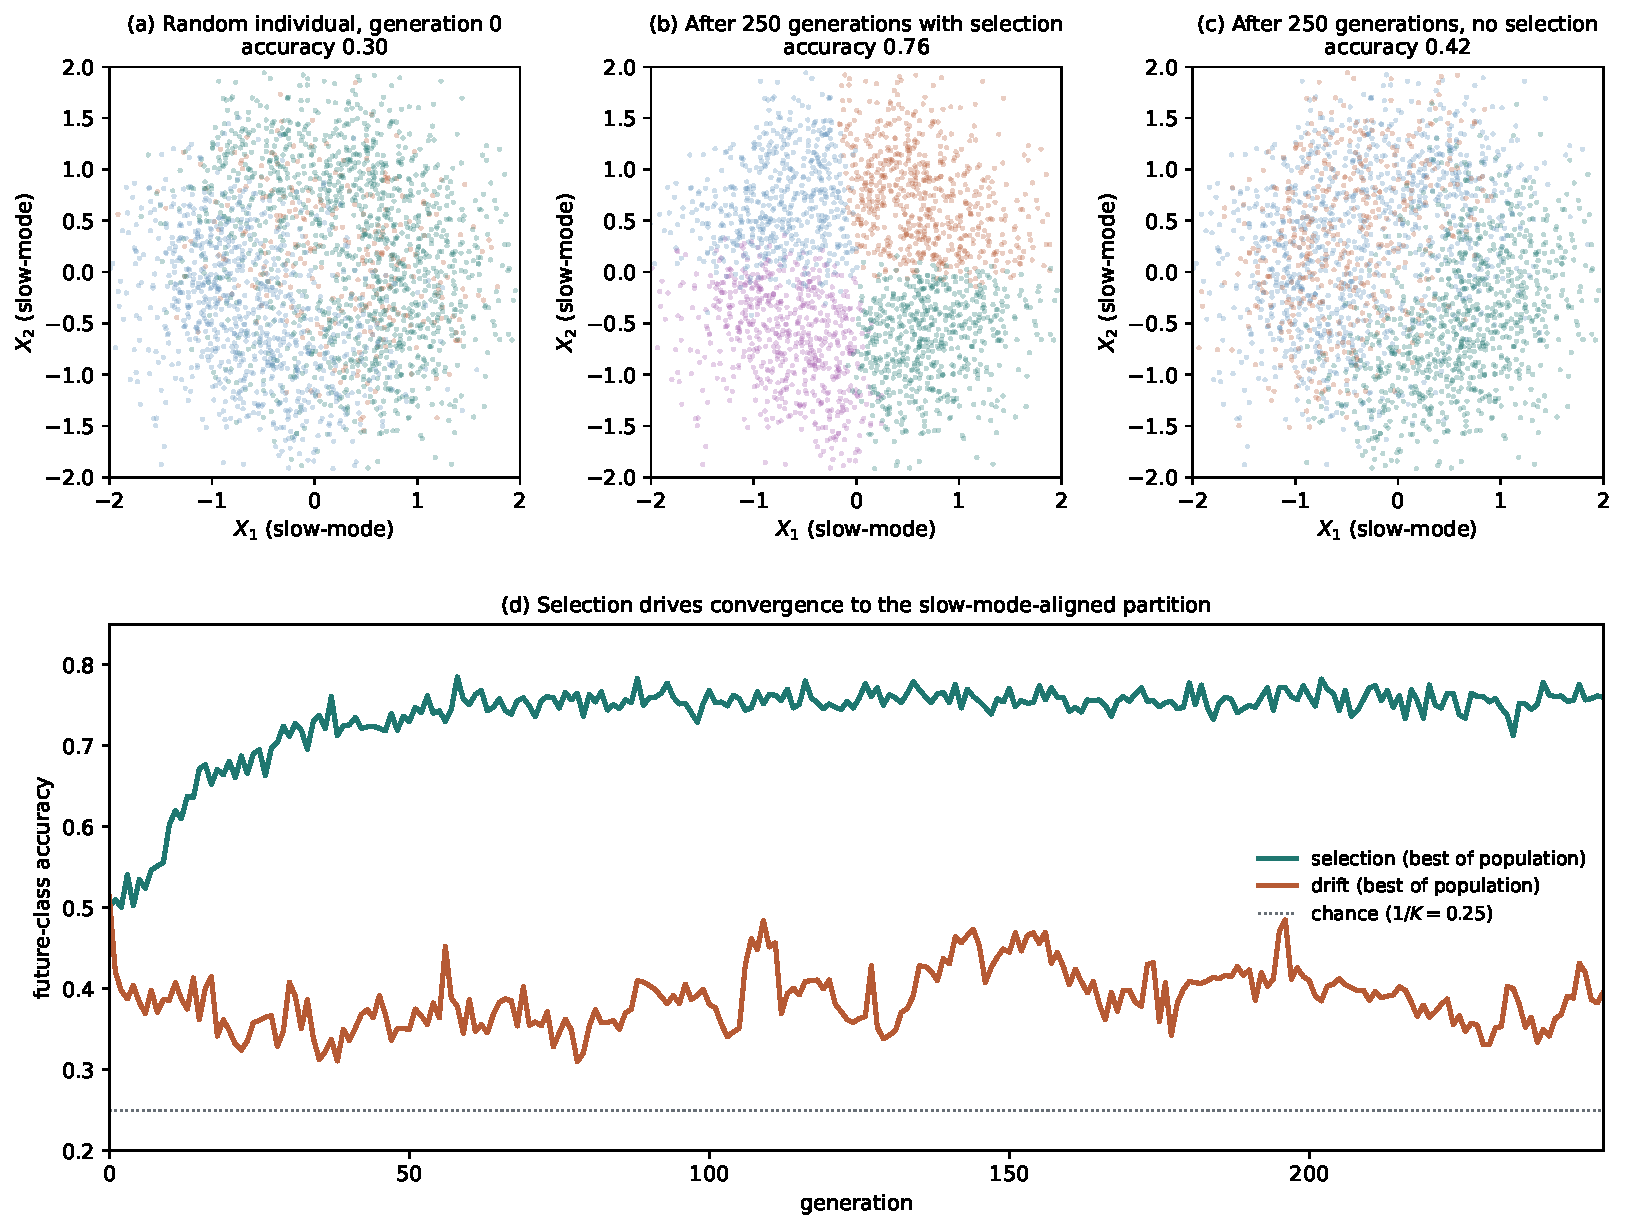
\includegraphics[width=\textwidth]{figures/fig3_emergence_demo.pdf}
\caption{Selection-driven boundary-code emergence. Substrate $X_t\in\R^6$ with slow-mode signal in two coordinates ($\sigma=0.45$) and Gaussian distractor noise in four ($\sigma=0.7$). $K=4$ codewords, population $64$, $250$ generations, top-half selection. (a) Generation $0$ random individual. (b) Best individual at generation $250$ under selection. (c) Best individual under drift control. (d) Future-class accuracy over generations; chance ($1/4$) and oracle ($1$) baselines dotted. Reproducible code in \texttt{simulations/emergence\_demo.py}. Robustness across nominal substrate dimension $N\in\{64,128,256,512\}$ (hidden nonlinear embedding of a $10$-dimensional latent slow trajectory) is reported in \texttt{simulations/first\_code\_complex\_sweep.py} and \texttt{figures/sweep\_N\_scaling.txt}: selection achieves normalized viability $0.66$--$0.78$ across the full $N$ range, robustly above the memoryless random-population baseline ($0.20$--$0.29$).}
\label{fig:emergence-demo}
\end{figure}

\subsection{A volumetric hourglass simulator}
\label{sec:volumetric}

The single-channel demonstration above hides the radial structure of real boundaries. To test the boundary-code principle in the setting actually present in biology, we run a multi-layer hourglass: a continuous high-dimensional bulk substrate, a chain of continuous Linear+$\tanh$ encoder layers progressively narrowing the representation, a single discrete waist with $K$ codewords (Gumbel--Softmax with straight-through estimation \citep{jang2017,maddison2017,vandenoord2017}), a chain of continuous decoder layers re-expanding the representation, and a final $R$-way classifier head. The continuous chain implements the radial coarse-graining; the discrete waist enforces the partition.

The substrate $X^{(0)}\in\R^{2048}$ is a fixed nonlinear embedding of a 16-dimensional latent state with four cyclic phase modes of distinct coherence times $\tau\in\{5,20,60,200\}$, four developmental drifts, and four Gaussian distractors. The future task $F_{t+\Delta}$ is the $R=8$-way octant index of the longest-coherence phase mode advanced by $\Delta=10$ time units; pointwise $\gamma$-action-incompatibility holds by construction with $\gamma=1$, $p=1/R$. The encoder--decoder width profile is $(2048,1024,512,256,128,64,32,16,32,64,128,256,512)$, with the waist at width 16. The waist alphabet $K$ is swept across $\{4,8,16,32,64,256,2048\}$ with 4--6 seeds per condition, trained 15{,}000 iterations by Adam (lr $=10^{-3}$, batch $=2048$). Per-iteration measurements include $D_{\rm eff}(r)$ at every continuous depth (participation ratio of the layer-state covariance), waist codeword-usage entropy $H(M_{\rm waist})$, $I(M_{\rm waist};F)$, and $I(M_{\rm waist};\phi_k)$ for each phase mode $k$. Reproducible code in \texttt{simulations/volumetric\_hourglass\_sim.py}.

\subsection{The cardinality floor binds at the waist}

Proposition~\ref{prop:forced} predicts that any low-regret protocol must use at least $r=R$ distinct reliable codewords; below that capacity, an explicit regret floor of $\gamma p$ acts. We test this by sweeping the waist alphabet $K$ and reading off, for each seed, the peak achieved accuracy across training together with the effective alphabet $K_{\rm eff} = 2^{H(M_{\rm waist})}$ at that peak. Peak rather than final values are the relevant measure because Gumbel--Softmax with finite minimum temperature has a known late-stage collapse mode; peak captures the architecture's achievable capacity, while final reports where stochastic optimization landed.

The result (Figure~\ref{fig:volumetric_keff}) is the classification-specialized cardinality benchmark implied by Proposition~\ref{prop:forced}: across all 38 seeds, peak accuracy as a function of $K_{\rm eff}$ tracks the envelope $\min(K_{\rm eff}/R,\ \alpha)$ with task-intrinsic ceiling $\alpha\!\approx\!0.78$ set by phase-drift noise. Seeds with $K_{\rm eff}<R$ ride the cardinality floor, including all six $K=4$ seeds at peak accuracy $0.505\pm 0.005$ (predicted $0.5$). Seeds with $K_{\rm eff}\geq R$ saturate at the task limit. The nominal alphabet $K$ is uninformative once $K_{\rm eff}$ is read; the binding constraint is the codewords actually used. We say ``classification-specialized'' because Proposition~\ref{prop:forced} is stated for general $\gamma$-action-incompatibility, while the empirical envelope $\min(K_{\rm eff}/R, 1)$ is the special case for uniformly weighted $R$-way classification with $\gamma=1$, $p=1/R$, and lossless decoders.

\begin{figure}[H]
\centering
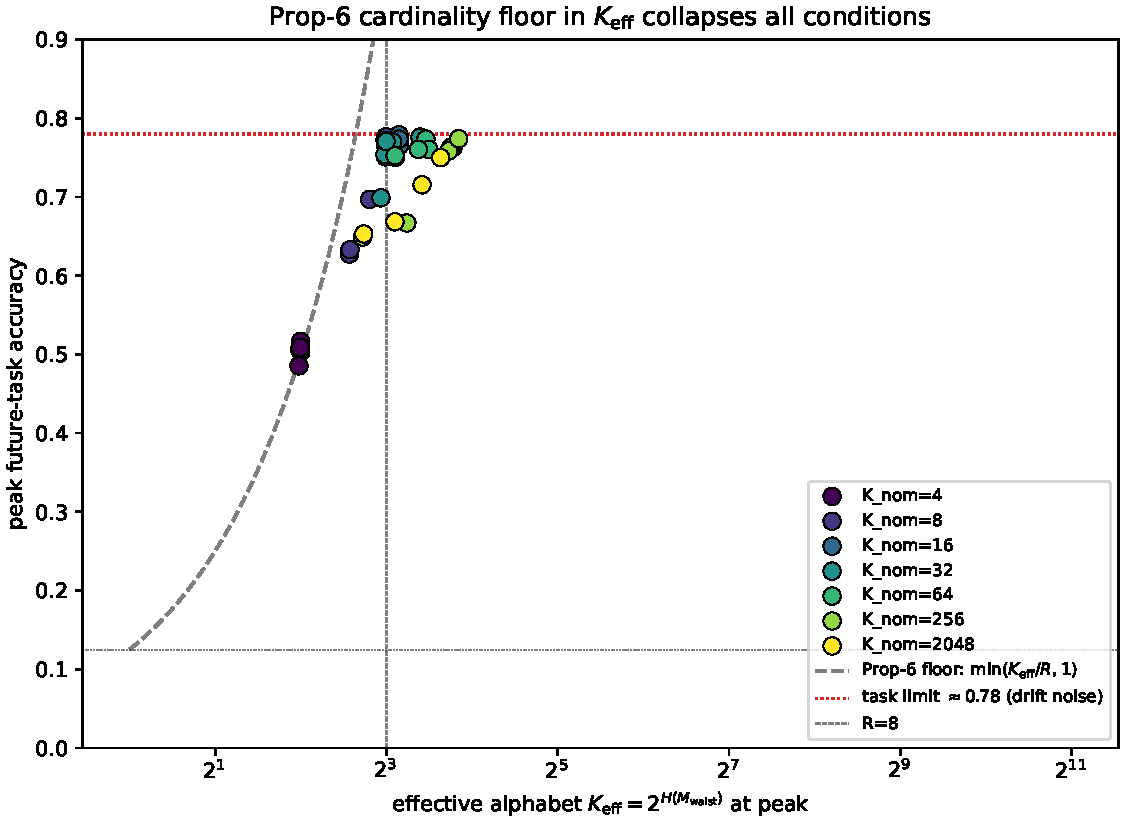
\includegraphics[width=0.78\textwidth]{figures/fig_volumetric_keff.pdf}
\caption{Classification-specialized cardinality benchmark: peak accuracy across nominal $K$ conditions tracks the same envelope when read in $K_{\rm eff}$. Each point is one seed's peak future-task accuracy plotted against the effective waist alphabet $K_{\rm eff}=2^{H(M_{\rm waist})}$ at peak. Seven nominal $K$ conditions (color), 4--6 seeds each, $R=8$. Dashed: the $\min(K_{\rm eff}/R, 1)$ envelope predicted by Proposition~\ref{prop:forced} specialized to uniformly-weighted $R$-way classification with $\gamma=1$, $p=1/R$. Dotted: task-intrinsic limit $\approx 0.78$ set by slow-mode drift noise. Below $K_{\rm eff}=R$ the floor binds tightly ($K=4$: $0.505\pm 0.005$, six seeds); above $R$, accuracy saturates at the task limit regardless of $K_{\rm nominal}$. Reproducible code in \texttt{simulations/volumetric\_hourglass\_sim.py}; analysis in \texttt{simulations/volumetric\_hourglass\_analyze.py}.}
\label{fig:volumetric_keff}
\end{figure}

The inefficient use of nominal capacity ($K_{\rm eff}\!\ll\!K$ for $K\gg R$) is itself informative: peak $K_{\rm eff}$ saturates near $R=8$ even at $K=2048$, with $K_{\rm eff}/K$ decreasing as $1/K$ for the larger conditions. This is the corollary that the channel sets an upper bound on the codebook (Corollary~\ref{cor:cardinality}), but selection on viability extracts only the codes the task can use. ``Excess capacity, sparse usage'' is the predicted regime when $K\gg R$.

\subsection{Volumetric collapse and partial re-expansion}

Beyond the cardinality result, the simulator makes the radial structure that a sharp-boundary idealization hides directly visible. Figure~\ref{fig:volumetric_radial} shows $D_{\rm eff}(r)$ at the per-seed peak-accuracy iteration, averaged across seeds. The bulk has $D_{\rm eff}\!\approx\!51$, consistent with the participation ratio of the $2048$-dimensional embedding's effective rank. Through the encoder, $D_{\rm eff}$ falls smoothly: $51\to 16\to 3.3\to 2.8\to\ldots\to 2.5\to 2.6$ at the waist, contracting more than an order of magnitude. The last few encoder layers and the waist itself sit at $D_{\rm eff}\!\approx\!2$--$3$. (The bare numerical coincidence between this $D_{\rm eff}$ value and $\log_2 R\!\approx\!3$ is not a quantitative match: $D_{\rm eff}$ is a participation ratio in linear units, while $\log_2 R$ counts bits; the relevant claim is that the post-collapse representation has only a handful of effective dimensions, not that those two quantities are equal.) Re-expansion is partial: the first decoder layer transiently raises $D_{\rm eff}$ to $\approx 5$, but subsequent layers do not recover bulk-level dimensionality.

\begin{figure}[H]
\centering
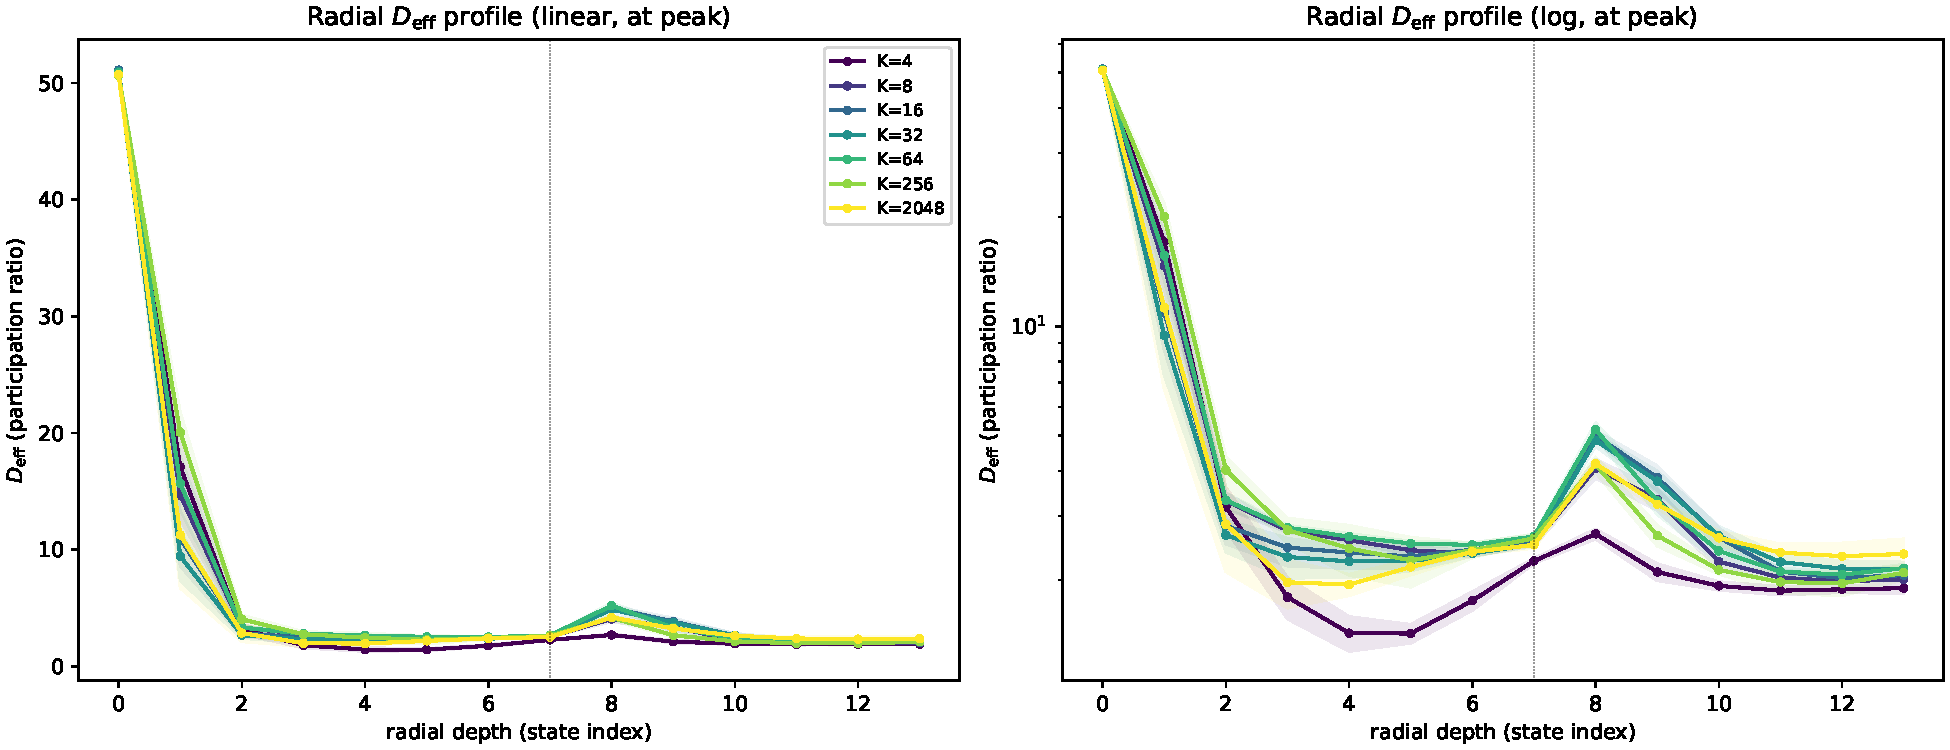
\includegraphics[width=\textwidth]{figures/fig_volumetric_radial.pdf}
\caption{Volumetric collapse and partial re-expansion. Mean $D_{\rm eff}(r)$ at peak across seeds, all seven $K$ conditions. Linear (left) and log (right) ordinates. The vertical dotted line marks the waist (depth 7). The bulk is high-$D$ ($\approx 51$); the encoder smoothly compresses through $\approx 16,3.3,2.8$ down to a waist of $\approx 2$--$3$; the decoder transiently re-expands but does not recover bulk dimensionality. The discrete waist breaks reversibility: information discarded by the projection cannot be recovered (Lemma~\ref{lem:nonrecoverability}), so post-waist $D_{\rm eff}$ is bounded by the available codebook structure rather than the substrate.}
\label{fig:volumetric_radial}
\end{figure}

Two predictions are confirmed by this profile. First, the boundary is volumetric, not sharp: the partition forms over a region of several layers in which $D_{\rm eff}$ is comparable to or below the rate-distortion floor, not at a single mathematical point. Second, the post-waist representation does not restore the bulk: by Lemma~\ref{lem:cascade}, the accessible information about any task-relevant variable is bounded above by its value at the waist on every decoder-side layer, regardless of how the receiver-side covariance rank evolves. The empirical post-waist $D_{\rm eff}$ rebound from $\approx 2.6$ to $\approx 5$ at depth 8 is therefore consistent with the cascade theorem: representational rank can grow downstream of the waist, but task-relevant distinctions absent from the waist message cannot be recovered. ``Shadow complexity'' (Corollary~\ref{cor:shadow}) is observable as the gap between bulk $D_{\rm eff}$ and post-waist $D_{\rm eff}$: $\approx 50\to 5$ in this run.

\subsection{Long-coherence slow modes survive deepest}

The last test isolates Proposition~\ref{prop:anticipation}'s prediction in the multi-mode case: when the substrate carries several slow modes, the waist should preserve only those whose phase the task's future loss depends on. Our design has four cyclic phase modes with coherence times $\tau\in\{5,20,60,200\}$, and $F_{t+\Delta}$ is constructed so that only $\phi_3$ (the $\tau=200$ mode) is task-relevant. Task relevance and coherence time are therefore confounded by construction; the test below speaks directly to the task-relevance dissociation but does not separately speak to a coherence-time-among-relevant-modes ranking. Figure~\ref{fig:volumetric_phase} reads off $I(M_{\rm waist};\phi_k)$ at the per-seed peak iteration for each of the four phase modes across all conditions.

\begin{figure}[H]
\centering
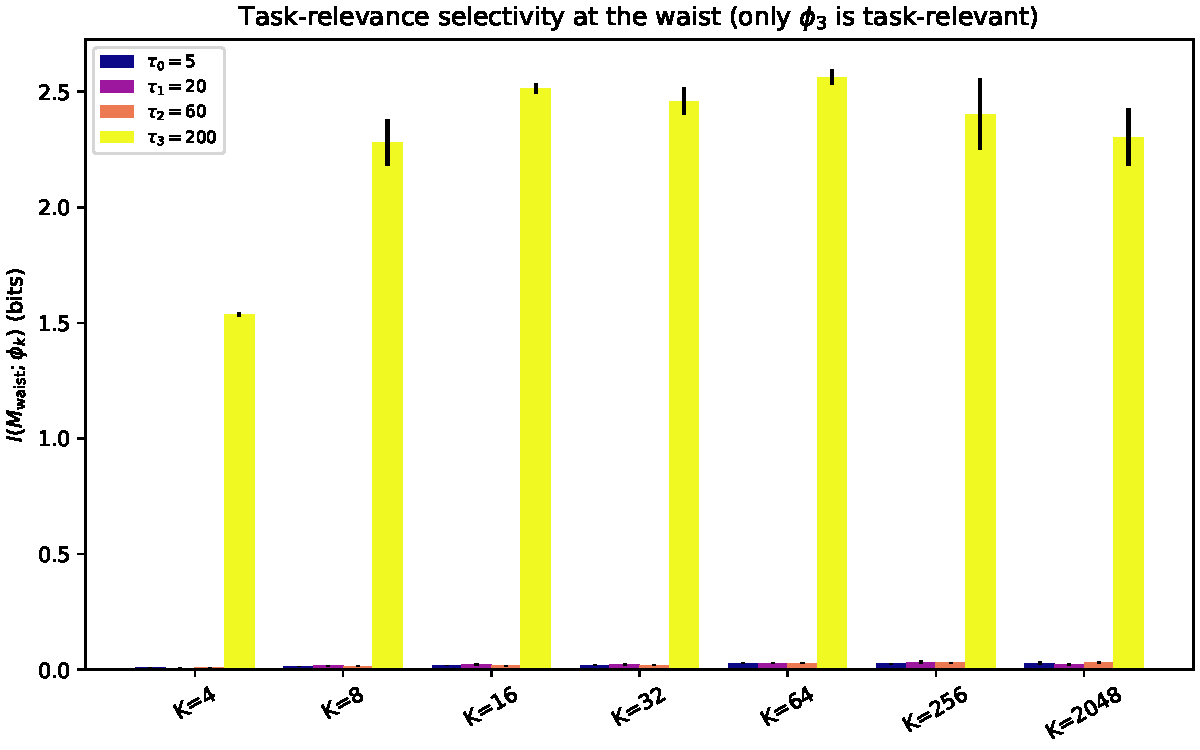
\includegraphics[width=0.78\textwidth]{figures/fig_volumetric_phase.pdf}
\caption{Task-relevance selectivity at the waist. $I(M_{\rm waist};\phi_k)$ at the per-seed peak iteration for each of four phase modes $k\in\{0,1,2,3\}$ with coherence times $\tau\in\{5,20,60,200\}$, mean and SEM across seeds, per nominal $K$. Only $\phi_3$ is task-relevant in this design (and is also the longest-coherence mode; relevance and coherence are confounded here). The waist preserves $\phi_3$ across all $K$ while the three task-irrelevant modes are aliased away. The waist functions as a task-driven slow-mode filter, retaining the trajectory class that constrains future loss and discarding the rest, consistent with Propositions~\ref{prop:anticipation}--\ref{prop:latent}.}
\label{fig:volumetric_phase}
\end{figure}

The dissociation is sharp. At $K=64$, $I(M_{\rm waist};\phi_3)=2.56\pm 0.03$ bits (peak iteration, six seeds), while $I(M_{\rm waist};\phi_{0,1,2})=0.028\pm 0.002$ bits each. The factor of $\approx\!90$ between the task-relevant mode and the task-irrelevant modes is observed at every $K$. This is the empirical version of the prediction in Section~\ref{sec:predictions}: a phase-disrupted preparation should impair anticipation while leaving present-state classification approximately intact. Here the waist is doing exactly this --- preserving the slow trajectory class that gates future loss, ignoring the rest. Operationally, the strongest biological codes should look the same: their boundary messages preserve the trajectory information that downstream loss depends on, and aliase modes that contribute no anticipatory horizon. A separate experiment varying coherence time \emph{among} task-relevant modes would be needed to test whether longer-coherence trajectory information is preserved preferentially when several relevant modes are simultaneously present.

\subsection{Additional demonstrations}

Two supporting numerical demonstrations from the earlier single-channel setup remain in the codebase. A bulk-channel ablation (decoder receives codeword, low-dimensional bulk context, both, or both with bulk shuffled at evaluation) supports the latent-context route of Proposition~\ref{prop:latent}: destroying bulk--environment synchronization at evaluation while preserving codeword identity collapses the synchronization-dependent viability while leaving a code-only architecture unaffected (\texttt{simulations/code\_vs\_bulk\_ablation.py}). A coupled-Kuramoto exploratory demonstration of stochastic-resonance-mediated synchronization (\texttt{simulations/stochastic\_resonance\_sweep.py}) is included as a minimal mechanism rather than a clean isolation; in its as-shipped configuration the no-code baseline retains residual phase-locking via frequency matching, so it illustrates the synchronization shape rather than quantifying the codeword's contribution.

\section{Mechanism}
\label{sec:mechanism}

The formal result gives the abstract form of code formation; biology implements it with thresholds, attractors, adapters, and interpreters. Three concrete mechanisms illustrate how viability pressure reshapes a partition.

\paragraph{Synaptic plasticity.} In Hebbian and reinforcement-modulated plasticity, distinct upstream microstates that demand the same action collapse onto a shared response, while microstates that demand different actions are pulled apart. Spike-pattern codes, place-cell codes, and motor-cortical decision codes can be read in this light \citep{buzsaki2004,fries2015,panzeri2010}.

\paragraph{Affinity maturation.} B-cell affinity maturation iteratively mutates antibody-binding regions and selects clones whose recognition aligns with downstream protective response \citep{janeway2001,davis1998}. Antigens with shared protective consequences collapse onto cross-reactive fibers; antigens whose downstream consequences diverge are split.

\paragraph{Morphogen-threshold sharpening.} Cell fate commitment converts continuous morphogen concentrations into discrete cell types via gene-regulatory bistability. Selection on robustness sharpens thresholds against noise and aligns them with action-relevant regimes \citep{pezzulo2016,levin2023,levin2025multiscale}.

In each case, three ingredients coincide: variation in encoder or decoder, a viability signal sensitive to within-fiber action mismatch, and a feedback path that reshapes the partition. Code formation is therefore co-adaptation of encoder and decoder at a boundary, not the appearance of a naked symbol list \citep{pattee2001,barbieri2003,barbieri2015}. The codeword does not contain the downstream dynamics; it selects or biases them. A side-effect with biological importance is that an internal update depending on $X$ only through $M$ is insulated from within-fiber environmental variation: codes convert unbounded environmental variation into a finite set of action-relevant categories, which is the formal sense in which they stabilize organisms against perturbation \citep{maturana1980}.

\section{Biological cases}
\label{sec:cases}

Table~\ref{tab:cases} fixes operational anchors for canonical biological codes. The same boundary-code logic appears across substrates with substrate-specific instantiations.

\begin{table}[H]
\centering
\small
\newcolumntype{L}[1]{>{\raggedright\arraybackslash}p{#1}}
\begin{tabular}{L{1.8cm}L{2.0cm}L{2.3cm}L{2.7cm}L{2.4cm}L{2.4cm}}
\toprule
\textbf{Case} & \textbf{Boundary} & \textbf{Message} & \textbf{Decoder} & \textbf{Slow mode} & \textbf{Failure mode} \\
\midrule
Genetic & germline & codon & tRNA adapter & lineage trajectory & misreading \\
Neural (long-range) & axon, synapse & spike pattern & postsynaptic dynamics & cortical oscillation & timing aliasing \\
Circadian / metabolic & cell--organism & molecule + phase & phase-gated expression & circadian cycle & mistiming \\
Morpho\-genetic & cell--tissue & cell-fate label & gene-regulatory bistability & developmental stage & patterning error \\
Immune & cell surface & MHC--peptide & T/B receptor & infection / repair phase & auto\-immunity \\
Endocrine / quorum & circulation & hormone regime & receptor cascade & density / cycle phase & desensit\-ization \\
Behavioral / social & body--observer & gesture, display & receiver policy & social cycle & mis\-coordination \\
\bottomrule
\end{tabular}
\caption{Operational anchors for biological codes. Each row identifies the substrate boundary, the codeword as physically realized, the decoder, the slow mode (if any) supplying anticipatory horizon, and one representative partition-failure mode.}
\label{tab:cases}
\end{table}

\paragraph{Genetic.} The framework does not derive the codon table; it explains why a finite codon--amino-acid mapping is expected at all. Generational coordination is an extreme dimensional boundary: the parent chemical system cannot transmit its full state, so it transmits a compressed reusable alphabet whose interpreter reanimates protein dynamics in the offspring \citep{crick1968,maynardsmith1995,barbieri2003}. The principle also speaks to origins, since its three ingredients --- high-dimensional substrate, finite-bandwidth interface, viability pressure --- do not require a mature symbolic adapter; the decoder $\delta$ can be any physical mechanism converting a thresholded interface state into a downstream effect, including autocatalytic thresholds and gating events available in early biology.

\paragraph{Neural.} Where timing and phase are directly accessible through local coupling, neural coding remains continuous. Where conduction distance, noise, and synaptic bottlenecks limit access, finite events and reusable spike patterns emerge \citep{buzsaki2004,fries2015,panzeri2010}. Spike identity alone is not the full code: phase, synchrony, and burst timing expand the boundary alphabet when the receiver can preserve them \citep{fries2005,canolty2010,lundqvist2016,miller2018working,sterling2015}, and slow oscillations gate faster local assemblies, making neural codes anticipatory when fast events are phase-indexed to slower cycles.

\paragraph{Circadian and metabolic.} The circadian clock is the cleanest case of anticipation by synchronisation \citep{winfree2001,forger2017,pittendrigh1993,lowrey2004}: local cells are entrained to an organismal clock whose phase constrains future environmental states. The codeword is molecule-in-phase, not molecule alone, and the same logic holds at shorter (feeding--fasting) and longer (seasonal) scales.

\paragraph{Morphogenetic and bioelectric.} Discrete cell fates are stable partitions of the continuous developmental substrate \citep{pezzulo2016,levin2023,levin2025multiscale,hansali2025}: cell-fate labels are boundary messages produced by the high-dimensional bioelectric and signalling substrate, with each local decision made in relation to a slowly varying body-plan trajectory that does not yet fully exist.

\paragraph{Immune.} The immune interface compresses the cellular substrate into finite recognitional channels --- MHC--peptide complexes, co-stimulatory markers, cytokines, checkpoint and tissue-context cues \citep{janeway2001,davis1998}. Autoimmunity, evasion, and exhaustion are partition failures: substrate regimes that alias onto the same message, or decoders tuned to the wrong equivalence classes. Recognition is also stage-dependent.

\paragraph{Endocrine and quorum sensing.} Hormones and autoinducers compress tissue state and population density into circulating signals \citep{miller2001,bassler2002}; the boundary alphabet is the set of reliably distinguishable regimes (below threshold, near threshold, above threshold; pulse, sustained, oscillation), not the concentration continuum.

\paragraph{Behavioural and social.} Posture, vocalisation, gesture, language, and institutional categories compress high-dimensional internal state into finite displays. Each signal class is a boundary partition: many internal states map to the same signal because they admit a shared receiver response. The section is illustrative; the formal results constrain only the boundary structure.

\section{Predictions}
\label{sec:predictions}

\paragraph{Codes localize at dimensional boundaries, and channel changes reshape them.} Codes should appear where direct coupling cannot carry task-relevant substrate dynamics, and weaken where continuous coupling preserves those dynamics. The predicted gradient runs from continuous integration within tightly coupled local regimes to discrete codes across membranes, long axons, developmental commitments, immune interfaces, generations, and organismal boundaries. If a boundary gains bandwidth, its code should soften, become more graded, or be partially replaced by continuous coupling; reduced bandwidth or increased noise should produce coarser, more categorical codes.

\paragraph{Codewords preserve action-relevant invariants, not microscopic similarity.} A mature code groups substrate states by downstream consequence. Molecularly different states may map to the same response if they admit the same protective action; molecularly similar states may be split if downstream consequences diverge. The correct test of a biological code is therefore not whether codeword classes are microscopically homogeneous, but whether each fiber is coherent under its assigned response (Definition~\ref{def:fiber}). Apparent context-dependence is not a nuisance variable; when future loss depends on slow trajectories, effective codes preserve the relevant trajectory class, and the same signal will have different effects at different circadian phases, developmental stages, inflammatory phases, neural oscillatory phases, or ecological seasons.

\paragraph{Phase-disrupted codes lose horizon, not identity.} The framework predicts a sharp dissociation: disrupting slow-mode phase while preserving local substrate dynamics should selectively impair anticipation while leaving present-state classification largely intact. In a phase-disrupted preparation (misaligned light--dark cycle, jet-lag protocol, sleep--wake fragmentation, scrambled developmental cue order), codeword identity at the moment of measurement should remain similar to control, but performance on tasks whose loss depends on future variables should drop disproportionately. Quantitatively, $\I((M,C);F_{t+\Delta})$ should drop toward the context-free baseline $\I(M;F_{t+\Delta})$, and toward zero in the pure latent-context regime, while $\I(M;Z_t)$ for present-state task variables should remain approximately preserved. By Proposition~\ref{prop:latent}, the relevant target of disruption is often the receiver's entrained context $C_t$ rather than the boundary message itself, so a clean test attacks $C_t$ while leaving $M_t$ intact. This dissociation is not predicted by accounts that treat codes purely as instantaneous classifiers. A clear comparison would measure immune recognition accuracy on stage-matched antigen tasks under intact vs.\ scrambled circadian phase, or neural decoding of present vs.\ future behavior in the same cortical population under intact vs.\ disrupted slow oscillations.

\paragraph{Anticipatory horizon scales with slow-mode coherence time.} The horizon of a code should scale with the coherence time of the longest task-relevant slow mode it preserves \citep{todd2026b_coherencetime}. A purely local chemical code coordinates immediate reactions; a circadian-anchored code anticipates day-scale transitions; a developmental code anticipates tissue-scale futures; a genetic code preserves lineage-scale constraints. A multi-mode substrate is predicted to filter the modes selectively: only those modes that gate future loss should be preserved through the waist; modes whose phase is irrelevant to viability should be aliased away, even if they are physically present in the bulk. Section~\ref{sec:emergence} confirms this directly: when the substrate carries four phase modes of distinct coherence times and only one is task-relevant, the boundary message preserves $\approx 90\times$ more information about the task-relevant mode than about the others, regardless of waist alphabet size.

\paragraph{Pathology is partition pathology.} Failures of regulation often take the form of partition errors. Too-coarse partitions produce aliasing; too-fine partitions produce fragmentation; decoder drift produces maladaptive interpretation; channel noise produces rigid defensive partitions because subtle distinctions cannot be safely transmitted. These are expected in immune disease, cancer immune evasion, developmental malformation, psychiatric rigidity, and institutional communication failures.

\paragraph{Higher-bandwidth observers reveal shadow structure.} A code hides within-fiber variation from receivers limited to it; better measurement should reveal structured variation inside codeword classes (Corollary~\ref{cor:shadow}). Single-cell sequencing reveals heterogeneity inside cell-type labels; high-resolution recording reveals timing structure inside firing-rate categories; spatial proteomics reveals immune-relevant structure inside coarse antigen classes. These discoveries should be expected, not treated as anomalies. The volumetric simulator (Section~\ref{sec:emergence}) makes the same point quantitatively: the receiver substrate's $D_{\rm eff}$ is bounded above by the waist alphabet, never recovering the bulk's high $D_{\rm eff}$, so any observable that the receiver pathway controls cannot in principle resolve all the structure that the sender bulk contains.

\section{Objections}
\label{sec:objections}

\paragraph{Is this just rate-distortion theory?} The formal core uses rate-distortion theory, but the biological claim is not merely rate-distortion. Standard rate-distortion theory assumes a source, distortion function, and code design problem. Biology supplies those ingredients physically: source as high-dimensional substrate, distortion as viability loss, channel as boundary, and code retention by selection, learning, plasticity, or development. The contribution is to identify biological code formation as the stable physical realization of this problem at dimensional boundaries, and to extend it across slow modes via Propositions~\ref{prop:anticipation}--\ref{prop:latent}.

\paragraph{Does this solve the genetic code?} No. It solves a prior problem: why a finite symbolic mapping is expected at the generational chemistry-to-protein boundary. The exact codon table reflects historical contingencies, chemical affinities, error minimization, stereochemical constraints, and frozen accidents \citep{crick1968,maynardsmith1995}.

\paragraph{Are all categories codes?} No. An external observer can categorize anything. A biological code must be used by the system or its coupled partner to coordinate action across a boundary. A cell type named by a scientist is not automatically a code; a cell-fate state that downstream tissues interpret during development is. The difference is endogenous use.

\paragraph{What about continuous signals?} Continuous signals can participate in codes when downstream interpretation partitions them into reliably distinguishable regimes. Many biological codes are mixed: continuous concentrations, timing, or phase relations are interpreted through thresholds, attractors, and competence windows. The principle predicts finite or effectively finite distinguishability at noisy finite-capacity boundaries, not literal digital discreteness at the substrate level.

\paragraph{Is anticipation just prediction?} No. Prediction usually means constructing an internal model of a future state; anticipation by synchronisation is weaker and more physical, supplying the future-conditioning by entrainment to a slow process rather than by an explicit model \citep{rosen1985,igamberdiev2014}.

\paragraph{How does this relate to active inference?} Active inference \citep{friston2010} describes how a system selects actions under a generative model; the boundary-code principle asks how finite message alphabets and interpretable partitions arise when the regulated substrate cannot cross the boundary in full. Codes are candidate physical implementations of the compressed, often slow-mode-indexed, sufficient statistics on which active inference operates.

\paragraph{Does slow-mode coupling make codes less discrete?} Yes, often: slow-mode-sensitive codes look less like static alphabets and more like alphabets indexed by context. Proposition~\ref{prop:latent} makes the operational unit the pair $(M_t,C_t)$, so an apparently phase-invariant boundary message can be perfectly anticipatory provided the receiver carries an entrained $C_t$.

\paragraph{Why is biology privileged if the principle is substrate-general?} The principle is substrate-general; what makes biology privileged is that retention is coupled to viability. In physics, projection across a boundary produces observables; in biology, projection plus retention pressure produces \emph{codes}. A living system preserves and interprets the projection because doing so sustains its own organization. Cosmological boundaries produce effective variables but no interpreter retains them; the result is observables, not codes. Biological boundaries produce interpreted alphabets because the interpreter is itself sustained by the partition working.

\paragraph{Does this prove all biological systems form codes?} Within the axiomatic framework of Section~\ref{sec:universal}, yes (Corollary~\ref{cor:calibrated}). Outside the framework, the claim is empirical: the axioms are independently motivated by five biological traditions, and the conditions are met at every substrate boundary in Section~\ref{sec:cases}. The contingent structure of any specific code (codon table, particular spike alphabets, cell-fate repertoires) is not derived; nor are systems violating Axiom~\ref{ax:nonequilibrium} (dormant spores under sufficient quiescence) covered, until they re-enter non-equilibrium maintenance.

\section{Relation to prior papers}
\label{sec:prior}

This paper continues a sequence on information-theoretic constraints in biological substrates. The falsifiability paper established that low-dimensional tests fail in high-dimensional biological systems near measurement thresholds \citep{todd2025falsifiability}; the timing-inaccessibility paper established that temporal order in continuous substrates cannot always be registered by finite observers without cost \citep{todd2025maxwell}; the intelligence paper established the high-dimensional-substrate / low-dimensional-interface architecture of living intelligence \citep{todd2026a_intelligence}; the coherence-time paper established that coordinated state registration has a rate limit in oscillator assemblies \citep{todd2026b_coherencetime}. The present paper asks what happens when such substrates must coordinate across boundaries and across timescales: code formation anchored to slow-mode synchronization.

\section{Conclusion}
\label{sec:conclusion}

Code formation is the stable solution to a boundary problem. High-dimensional biological substrates contain more task-relevant structure than finite channels can transmit. Direct state sharing fails. Downstream processing cannot recover distinctions that projection erased. Repeated selection on coordination success therefore stabilizes finite partitions of substrate state. A biological code is a reusable, interpreted, viability-coupled partition at a dimensional boundary. Where action-incompatible regimes recur, low-regret coordination is forced to assign them distinct reliable messages or incur an explicit regret floor. Within an axiomatization of bounded self-maintenance, any system satisfying the conditions forms at least one nontrivial code at at least one of its boundaries.

The strongest biological codes add two further properties. They preserve a slow-mode trajectory class --- in the message, in the receiver's entrained context, or in both --- so that a local system synchronised to a slow trajectory can act with respect to future constraints without simulating future microstates. And they live across a continuous radial region rather than at a mathematical surface: the cascade lemma (Lemma~\ref{lem:cascade}) plus Lemma~\ref{lem:projection} together imply that the partition crystallises at whatever depth the accessible task information first falls below the rate-distortion demand --- empirically accompanied by the observed $D_{\rm eff}$ collapse --- that decoder-side re-expansion can grow representational rank but not recover task-relevant distinctions, and that only the slow modes whose future loss the boundary is exposed to survive the waist. The simulator in Section~\ref{sec:emergence} makes all three signatures empirically visible.

In one line: a finite-bandwidth boundary does not merely compress a high-dimensional biological substrate; under viability-coupled recurrence, it converts the substrate into a finite action-sufficient partition, leaving the remaining internal degrees of freedom as within-codeword shadow complexity. This reframes biological codes as consequences of physical constraint rather than optional representational overlays. Genetic codons, neural spikes, circadian gates, morphogenetic fates, immune motifs, hormones, quorum signals, and behavioral displays differ mechanistically but solve the same abstract problem: how to coordinate across a boundary too narrow for the dynamics themselves. Where continuous coupling suffices, no code is needed. Where it fails, retained low-loss solutions take code-like form. Biology uses codes because boundaries force it to compress, and viability teaches the compression what to preserve.

\section*{Declarations}

\paragraph{Funding.} No specific funding was received for this work.

\paragraph{Competing interests.} The author declares no competing interests.

\paragraph{Data availability.} No empirical datasets were generated or analysed during the current study. The figures and worked examples are produced by deterministic simulation code with fixed RNG seeds; the code (\texttt{simulations/}) and exact numerical outputs (\texttt{figures/*.txt}) are included with the manuscript and are also available at \url{https://github.com/todd866/code-formation-biosystems}.

\paragraph{Author contributions.} Sole authorship.

\paragraph{Use of AI tools.} During preparation of this work the author used Anthropic Claude and OpenAI GPT-5-class models for drafting assistance, mathematical review, and manuscript editing. All claims, definitions, formal statements, proofs, and scientific positions were directed, verified, and approved by the author, who takes full responsibility for the content of this manuscript.

\appendix

\section{Methods for the simulations}
\label{app:methods}

This appendix describes the simulation pipeline behind Figures~\ref{fig:boundary-code}--\ref{fig:volumetric_phase} and the supporting bulk-channel and stochastic-resonance demonstrations referenced in Section~\ref{sec:emergence}. The single-channel demonstrations (Figures~\ref{fig:phase-demo}--\ref{fig:emergence-demo}) are deterministic NumPy + Matplotlib. The volumetric hourglass simulator (Figures~\ref{fig:volumetric_keff}--\ref{fig:volumetric_phase}) is implemented in PyTorch with the Apple Metal backend; it is deterministic given the script-level seeds modulo MPS reduction-order nondeterminism that affects only low-order digits of the metrics.

\paragraph{Single-channel demonstrations.} Figures~\ref{fig:phase-demo}--\ref{fig:emergence-demo} use a NumPy population-evolution setup. Two substrate families: a 6-dimensional toy world placing a slow phase $\phi_t\sim\mathrm{Unif}[0,2\pi)$ on the unit circle with $X_{1:2}=(\cos\phi_t,\sin\phi_t)+\eta_t$ plus four Gaussian distractors; and a hidden-embedding world (used in the supporting ablations below) lifting a 10-dimensional latent slow trajectory into a nominal $N$-dimensional substrate via a linear+quadratic+$\tanh$ embedding. The encoder $\pi_\theta:\R^N\to\{0,\ldots,K-1\}$ argmaxes $K$ linear projections; the decoder $\delta\in\{0,\ldots,R-1\}^K$ is a lookup table. A population of $P{=}64$--$160$ pairs is evolved for $G{=}250$--$450$ generations under top-fraction-$f{=}0.45$ selection on future-class accuracy, with Gaussian-noise mutants and occasional decoder-table flips. Two controls accompany selection: a fitness-blind drift baseline using the same mutation operator with random parents, and a memoryless random-population baseline (``random search'' in captions) that redraws the entire population each generation. Metrics: future-class accuracy, normalised viability (mean-action policy $0$ to oracle $1$), and codeword-usage entropy $H(M)/\log_2 K$. Hyperparameters and per-script configs in the simulation files.

\paragraph{Bulk-channel ablation and stochastic-resonance demonstration.} Two supporting demonstrations illustrate the latent-context route of Proposition~\ref{prop:latent}. The bulk-channel ablation evolves four architectures (\textsc{code-only}, \textsc{bulk-only}, \textsc{code+bulk}, \textsc{code+bulk trained shuffled}) and compares an intact pass on synchronised $(X,C,F)$ against a shuffled-eval pass that permutes the bulk context $C$ while preserving the codeword: \textsc{code+bulk} drops sharply under shuffled-eval while \textsc{code-only} is unaffected, the predicted synchronisation-collapse signature. The stochastic-resonance demonstration couples two Kuramoto-style networks $B_1,B_2$ through a discrete codeword $M_t$ that quartile-bins $B_1$'s mean phase, with a weak below-threshold environmental signal $E_t$ forcing $B_1$ and noise swept on a log grid. As shipped this is not a clean isolation of the codeword's contribution: the \textsc{no-code} baseline retains residual $B_2$-to-$E_{t+\Delta}$ phase-locking through intrinsic-frequency matching, so the demo illustrates the synchronisation shape rather than quantifying the codeword's effect. Full architectures, hyperparameters, and condition definitions live in \texttt{simulations/code\_vs\_bulk\_ablation.py} and \texttt{simulations/stochastic\_resonance\_sweep.py}.

\paragraph{Volumetric hourglass simulator.} A 16-dimensional latent state with four cyclic phase modes of distinct coherence times $\tau\in\{5,20,60,200\}$ (drift variance $\Delta/\tau$), four developmental drifts on $[-1,1]$, and four Gaussian distractors generates the substrate $X^{(0)}\in\R^{2048}$ via a fixed nonlinear lift $X^{(0)} = \tanh(W_2 \tanh(W_1 z) + W_3 \cdot \mathrm{vec}(zz^\top))$. The future task $F_{t+\Delta}$ with $\Delta=10$ is the $R=8$-way octant of the longest-coherence phase mode at $t+\Delta$ (pointwise $\gamma$-action-incompatibility with $\gamma=1$, $p=1/R$). The architecture is a chain of continuous Linear+$\tanh$ encoder layers with widths $(2048,1024,512,256,128,64,32,16)$, a single discrete Gumbel--Softmax waist of $K$ codewords (codebook embedding dim 16; straight-through estimator), continuous Linear+$\tanh$ decoder layers with widths $(16,32,64,128,256,512)$, and a final $R$-way Linear classifier. Adam (lr $10^{-3}$, batch $2048$, grad-norm clip $5$); Gumbel temperature anneals from $\tau=1.0$ to $\tau=0.5$ over the first 40\% of 15{,}000 iterations and is held constant thereafter. Six seeds for $K\in\{4,8,16,32,64\}$, four seeds for $K\in\{256,2048\}$. Per-iteration logging of $D_{\rm eff}(r)$ at every continuous depth, $H(M_{\rm waist})$, $I(M_{\rm waist};F)$, and $I(M_{\rm waist};\phi_k)$ for each phase mode. Implementation in PyTorch using \texttt{F.gumbel\_softmax}; run on Apple M5 MPS.

\paragraph{Peak vs final reporting.} For Figures~\ref{fig:volumetric_keff}--\ref{fig:volumetric_phase} we report quantities at the per-seed iteration of peak future-task accuracy. With finite $\tau_{\min}$, Gumbel--Softmax has a known late-stage collapse mode in which a converged solution drops a subset of its codes; \emph{peak} captures the architecture's achievable capacity (the relevant quantity for the rate-distortion question Proposition~\ref{prop:forced} is asking) while \emph{final} captures where stochastic optimisation eventually landed. Both are stored; figure captions identify which is shown. Across our run, even $K=4$ showed only a modest peak/final gap (mean peak $0.505$, mean final $0.455$), while higher-$K$ conditions had substantially wider gaps (e.g.\ $K=16$: mean peak $0.766$, mean final $0.370$).

\paragraph{Scripts and outputs.} Each main and supporting experiment maps to a script and a deterministic results file. Scripts fix RNG seeds in their config blocks.

{\sloppy
\begin{itemize}
\setlength\itemsep{0pt}
\item Fig.~\ref{fig:boundary-code} (forced codeword separation schematic): \\ \texttt{simulations/fig1\_schematic.py}.
\item Fig.~\ref{fig:phase-demo} (one-bit phase demo): \\ \texttt{simulations/generate\_figures.py}, \texttt{figures/phase\_partition\_results.txt}.
\item Fig.~\ref{fig:emergence-demo} (selection demo): \\ \texttt{simulations/emergence\_demo.py}, \texttt{figures/emergence\_results.txt}.
\item Figs.~\ref{fig:volumetric_keff}--\ref{fig:volumetric_phase} (volumetric hourglass): \\
  \texttt{simulations/volumetric\_hourglass\_sim.py}, \\
  \texttt{simulations/volumetric\_hourglass\_analyze.py}; \\
  per-condition aggregate histories under \texttt{runs/<ts>\_volumetric\_sweep/<condition>/}.
\item Bulk-channel ablation: \\
  \texttt{simulations/code\_vs\_bulk\_ablation.py}, \\ \texttt{figures/ablation\_code\_vs\_bulk.txt}.
\item Stochastic-resonance demo: \\
  \texttt{simulations/stochastic\_resonance\_sweep.py}, \\ \texttt{figures/stochastic\_resonance.txt}.
\end{itemize}
}

\bibliographystyle{plainnat}
\bibliography{references}

\end{document}
